\documentclass[fleqn,usenatbib]{mnras}

\usepackage{newtxtext,newtxmath}
\usepackage[T1]{fontenc}
\DeclareRobustCommand{\VAN}[3]{#2}
\let\VANthebibliography\thebibliography
\def\thebibliography{\DeclareRobustCommand{\VAN}[3]{##3}\VANthebibliography}


%%%%% PACKAGES %%%%%
\usepackage{amsmath}
\usepackage{graphicx}
\usepackage{enumitem}
\usepackage{xcolor}
\usepackage{hyperref}
\usepackage{gensymb}
\usepackage{CJK}
\usepackage{tabularx}
\usepackage{orcidlink}
\usepackage{fontawesome}
\usepackage[normalem]{ulem}
\hypersetup{
    unicode, 
    colorlinks=true,
    linkcolor=linkcolor,
    citecolor=linkcolor,
    filecolor=linkcolor,
    urlcolor=linkcolor,
}
\definecolor{linkcolor}{rgb}{0.0,0.3,0.5}

%%%%% COMMANDS %%%%%
\newcommand{\SB}[1]{{\textcolor{purple}{SB: #1}}}
\newcommand{\comment}[1]{\textcolor{lightgray}{#1}}

\newcommand{\asa}{\textcolor{teal}}
\newcommand{\asac}[1]{\color{teal}[ÁS: #1] \color{black}}
\newcommand{\asams}[1]{\textcolor{magenta}{\sout{#1}}}
\newcommand{\asam}{\textcolor{magenta}}
\newcommand{\asas}[1]{\textcolor{teal}{\sout{#1}}}

\newcommand{\mkn}[1]{\textbf{\textcolor{blue}{MKN: #1}}}

%%%%%%%%%%%%%%%%%%%%%%%%%%%%%%%%%%%%%%%%%%%%%%%%%
%%%%%%%%%%%%%%%%%%%%%%%%%%%%%%%%%%%%%%%%%%%%%%%%%
% \begin{document}
\title[A golden thread through time and space I]{A golden thread through time and space: The chemodynamical memory of a major merger in a simulated NIHAO-UHD Milky Way analogue I\thanks{NIHAO-UHD is the Ultra High Definition re-run of a Milky Way analogue from the \textit{Numerical Investigation of a Hundred Astronomical Objects} (NIHAO) suite \citep{Wang2015}.}}

\author[S. Buder et al.]{Sven Buder,$^{1}$\thanks{E-mail: sven.buder@anu.edu.au}\thanks{Australian Research Council DECRA Fellow}\orcidlink{0000-0002-4031-8553}
Tobias Buck,$^{2,3}$\orcidlink{0000-0003-2027-399X}
Ása Skúladóttir,$^{4}$\orcidlink{0000-0001-9155-9018}
Melissa Ness,$^{1}$\orcidlink{0000-0001-5082-6693}
Madeleine McKenzie,$^{5}$\thanks{NASA Hubble Fellow}\orcidlink{0000-0002-1715-1257}
and\newauthor
Stephanie Monty$^{6, 7}$\orcidlink{0000-0002-9225-5822}
\\
$^{1}$Research School of Astronomy and Astrophysics, Australian National University, Canberra, ACT 2611, Australia\\
$^{2}$Universit{\"a}t Heidelberg, Interdisziplin{\"a}res Zentrum f{\"u}r Wissenschaftliches Rechnen, Im Neuenheimer Feld 205, D-69120 Heidelberg, Germany\\
$^{3}$Universit{\"a}t Heidelberg, Zentrum f{\"u}r Astronomie, Institut f{\"u}r Theoretische Astrophysik, Albert-Ueberle-Straße 2, D-69120 Heidelberg, Germany\\
$^{4}$Dipartimento di Fisica e Astronomia, Universitá degli Studi di Firenze, Via G. Sansone 1, I-50019 Sesto Fiorentino, Italy\\
$^{5}$The Observatories of the Carnegie Institution for Science, 813 Santa Barbara Street, Pasadena, 91101, CA, USA\\
$^{6}$Institute of Astronomy, University of Cambridge, Madingley Road, Cambridge CB3 0HA, UK\\
$^{7}$Department of Astronomy, New Mexico State University, Las Cruces, NM 88003, USA
}

% These dates will be filled out by the publisher
\date{Accepted DD MM 2025. Received DD MM 2025; in original form DD MM 2025}

% Prints the current year, for the copyright statements etc. To achieve a fixed year, replace the expression with a number. 
\pubyear{\the\year{}}

% Don't change these lines
\begin{document}
\label{firstpage}
\pagerange{\pageref{firstpage}--\pageref{lastpage}}
\maketitle

\begin{abstract} % 249 words, 1708 characters with space
%Understanding how the Milky Way's present-day structure — including its thin and thick disc populations — was shaped by processes such as past major mergers is a key goal of galactic archaeology. The chemical and dynamical structure of the Milky Way retains the imprint of such ancient events, including a major accretion episode around 8–10 Gyr ago. Recent findings suggest that present-day orbital energy correlates with stellar chemistry and birth location within the merging progenitor galaxy. Using a high-resolution, cosmological zoom-in NIHAO-UHD simulation of a Milky Way analogue, we trace the birth positions, ages, and present-day orbits of stars accreted in its last major merger. Comparing birth and present-day positions of older in-situ stars, we find negligible splashing/heating of their stellar orbits. Stars born in the accreted galaxy’s core are more tightly bound to the Milky Way and element-enhanced, while those from the outskirts are more weakly bound and less chemically enriched. This supports the scenario proposed by Skúladóttir et al. (2025) using idealised N-body simulations, now demonstrated in a cosmological context. The chemodynamical evolution within the accreted galaxy is also evident in elemental planes such as [Al/Fe] vs. [Mg/Mn], reflecting gradients in star formation efficiency and history. Our results reveal that spatial and temporal memory is preserved across the merger -- connecting birth locations to present-day properties like a golden thread. These findings imply that selecting only stars with higher orbital energies or radial actions risks systematically biased reconstructions of the progenitor galaxy, underestimating its total stellar mass, chemical enrichment, and role in shaping the early Milky Way.
Understanding how the Milky Way's present-day structure was shaped by past major mergers is a key goal of galactic archaeology. The chemical and dynamical structure of the Galaxy retains the imprint of such events, including a major accretion episode around 8--10~Gyr ago. Recent findings suggest that present-day orbital energy correlates with stellar chemistry and birth location within the merging progenitor galaxy. Using a high-resolution NIHAO-UHD cosmological zoom-in simulation of a Milky Way analogue, we trace the birth positions, ages, and present-day orbits of stars accreted in its last major merger. We show that stars born in the progenitor’s core are more tightly bound to the Milky Way and chemically enriched, while those from the outskirts are less bound and metal-poor. This supports the scenario proposed by Skúladóttir et al. (2025) using idealised simulations, now demonstrated in a cosmological context. The preserved chemodynamical memory is also evident in elemental planes such as [Al/Fe] vs. [Mg/Mn], reflecting gradients in star formation efficiency. Our results reveal that spatial and temporal memory is retained across the merger — connecting birth locations to present-day properties like a golden thread. We demonstrate that selection methods in integrals-of-motion space systematically bias progenitor reconstructions by missing its enriched core, and we outline strategies to obtain a more representative census of accreted stars.
\end{abstract}

\begin{keywords}
% {
Galaxy: evolution -- Galaxy: formation -- Galaxy: structure -- Galaxy: abundances -- Galaxy: kinematics and dynamics
% }
\end{keywords}

% \maketitle

%%%%%%%%%%%%%%%%%%%%%%%%%%%%%%%%%%%%%%%%%%%%%%%%%
%%%%%%%%%%%%%%%%%%%%%%%%%%%%%%%%%%%%%%%%%%%%%%%%%
\section{Introduction}
\label{sec:introduction}

Understanding what shaped the Milky Way and its present-day structure remains a central goal of galactic archaeology \citep{FreemanBlandHawthorn2002,BlandHawthorn_Gerhard2016}. The discovery of the thin and thick disc components \citep{Yoshii1982, Gilmore1983}, characterised by their largely distinct spatial, chemical and age distributions \citep[for example][]{Bensby2014, Hayden2015}, has led to numerous formation scenarios being proposed. These include turbulent high-redshift star formation producing a kinematically hot thick disc \citep{Bird2013, Stinson2013}, internal heating and radial migration within an evolving disc \citep{Schoenrich2009, Minchev2013, Sharma2021b}, a strong sensitivity of star formation to temporarily lower gas accretion \citep{Grand2018, Orkney2025}, as well as gas-rich mergers \citep{Brook2004, Buck2020} and the build-up of the disc under a two-infall scenario \citep{Chiappini1997, Spitoni2019}. More and more likely is seems to actually be a combination of multiple pathways \citep[e.g.][]{Orkney2025}.

Thanks to new observations of the \textit{Gaia} satellite \citep{Brown2021b} and spectroscopic follow-up it has become evident that the Milky Way's halo is built from numerous substructures, providing clear signatures of both past and ongoing accretion events \citep{Belokurov2006, Myeong2018c, Koppelman2019, Naidu2020, Yuan2020, Dodd2023}. One particularly influential finding is that a major merger (hereafter called \textit{GSE}) with an estimated mass ratio between 1:2.5 and 1:4 \citep{Helmi2018, Naidu2020} occurred roughly 8–10~billion years ago, somewhat disrupting the protodisc and certainly contributing significantly to the halo. Early hints of this event came from stellar abundance patterns \citep{Nissen2010}, and were later confirmed with significant dynamical information from the \textit{Gaia} mission \citep{Brown2016, Brown2018} by \citet{Belokurov2018} and \citet{Helmi2018}, giving new weight to the proposed gas-rich merger hypothesis.

As summarised by \citet{Helmi2020}, the focus has now shifted from merely identifying accreted stars to characterising the properties of the merging progenitor galaxy and its gas content. Several studies have investigated its global chemical composition \citep[for example][]{Das2020, Feuillet2021, Aguado2021, Matsuno2021, Buder2022, Belokurov2022, DeSilva2023, Monty2024, Ou2024}, while others tried to recover the merger process itself \citep[for example][]{Naidu2021} as well as the effects of the merger on the existing stars, such as the \textit{splashing} of stars \citep{Belokurov2020, Belokurov2022}. More recently, \citet{Skuladottir2025}, building on N-body simulations by \citet{Mori2024}, examined how chemical properties vary with orbital characteristics. Even with fewer than one hundred stars in their updated sample from \citet{Nissen2010, Nissen2024}, they successfully separated the accreted stars into more and less bound populations through more or less negative orbit energies and identified statistically significant chemical differences between them. \citet{Skuladottir2025} interpreted these trends using the scenario proposed by \citet{Mori2024}, in which the outer stars of the accreted galaxy—characterised by higher (less negative) orbital energies—were accreted earlier and at larger Galactocentric radii, while stars from the central regions, with lower (more negative) energies, were accreted later and more centrally. The inferred radial gradient in star formation efficiency led to systematically higher $\mathrm{[Fe/H]}$ and $\mathrm{[Mg/Fe]}$ abundances in stars formed in the former core of the galaxy, a picture consistent with observations of present-day dwarf galaxies (Lucchesi et al. in prep).

To further test and refine this scenario, we turn to a different simulation suite: the NIHAO-UHD project, which provides high-resolution, fully cosmological zoom-in simulations of Milky Way-type galaxies undergoing satellite accretion \citep{Buck2020, Buck2020b, Buck2021}. Unlike the idealised N-body simulations by \citet{Mori2024}, NIHAO-UHD self-consistently models the chemical and dynamical evolution of stars within a hierarchical cosmological context \citep{Buck2021}. 
The simulation in particular also includes two post-processing steps that make it particularly well suited to study the chemodynamical memory of the galaxy and its major mergers. Firstly, we have traced the birth positions of stars in discrete $100\,\mathrm{Myr}$ time steps, enabling a clean separation of in-situ from accreted stars\footnote{Potential inaccuracies arise around the time of the major merger itself.}. Secondly, we have calculated the same integrals of motion, that is orbit energies and actions for the Milky Way analogue simulation that are calculated for stars in our Milky Way galaxy.

In this first paper (Paper I) of the series we address the following questions: 
\begin{enumerate}[leftmargin=2em,labelwidth=0em]
    \item What can we learn about the selection efficiency of accreted stars in integrals of motions phase-space \citep{Helmi2018, Feuillet2021, Buder2022, Monty2024}?
    \item What memory of the birth positions and past chemical evolution is retained in integrals of motion space \citep{Skuladottir2025}?
%    \item How do the effects of the merger process manifest in the simulation, for example through the proposed \textit{splashing} of in-situ star orbits \citep{Belokurov2020} or mixing of in-situ and accreted gas to form \textit{splashed} stars?
\end{enumerate}

Paper II analyses, how the effects of the merger process manifest in the simulation, for example through the proposed \textit{splashing} of in-situ star orbits \citep{Belokurov2020} or mixing of in-situ and accreted gas to form \textit{splashed} stars.

By answering these questions with a Milky Way analogue simulation, we reveal a preserved chemodynamical memory of the last major merger and unveil connections and biases that fundamentally change how we reconstruct the Milky Way's formative history.

%%%%%%%%%%%%%%%%%%%%%%%%%%%%%%%%%%%%%%%%%%%%%%%%%
%%%%%%%%%%%%%%%%%%%%%%%%%%%%%%%%%%%%%%%%%%%%%%%%%
\section{Simulated data} \label{sec:data}

In this study we examine the high-resolution cosmological zoom-in simulation \texttt{g8.26e11}, a Milky Way analogue from the \textit{Numerical Investigation of a Hundred Astronomical Objects} (NIHAO) simulation suite \citep{Wang2015} that includes newly available chemical-evolution tracing.
We use \texttt{g8.26e11} because, as described below, it closely matches several key Milky Way properties — halo and stellar mass, rotation curve, and a disk-dominated, multi-armed spiral morphology — and experienced a major merger at a lookback time comparable to the Milky Way's last major merger.
Although the model does not form a strong bar \citep[see][]{Buder2025}, we argue that this is not critical for the questions addressed here.

This galaxy model forms part of the NIHAO-UHD series \citep{Buck2020b} and has been utilised in several prior investigations, including work on the properties of Milky Way satellites \citep{Buck2019b}, the spin of the Galactic dark matter halo \citep{Obreja2022}, abundance clustering to reconstruct birth conditions of stars \citep{Ratcliffe2022}, and the redshift evolution as well as shape of radial metallicity gradients in the ISM \citep{Ratcliffe2025, Buder2025}. A version of this simulation with reduced mass resolution was also employed by \citet{Buck2023} and \citet{Buder2024} to explore the chemical tagging of stars associated with its last significant accretion event (\textit{GSE}).

We briefly describe the simulation with reference to the above mentioned works in Sec.~\ref{sec:data_simulation}. The main new insights for this simulation are provided by additional information on the birth positions of star particles (see Fig.~\ref{fig:tracing_insitu_accretion_2}) as well as orbit properties, which we describe in Secs.~\ref{sec:data_birth_positions} and \ref{sec:data_orbit_properties}, respectively.

\begin{figure}
    \centering
    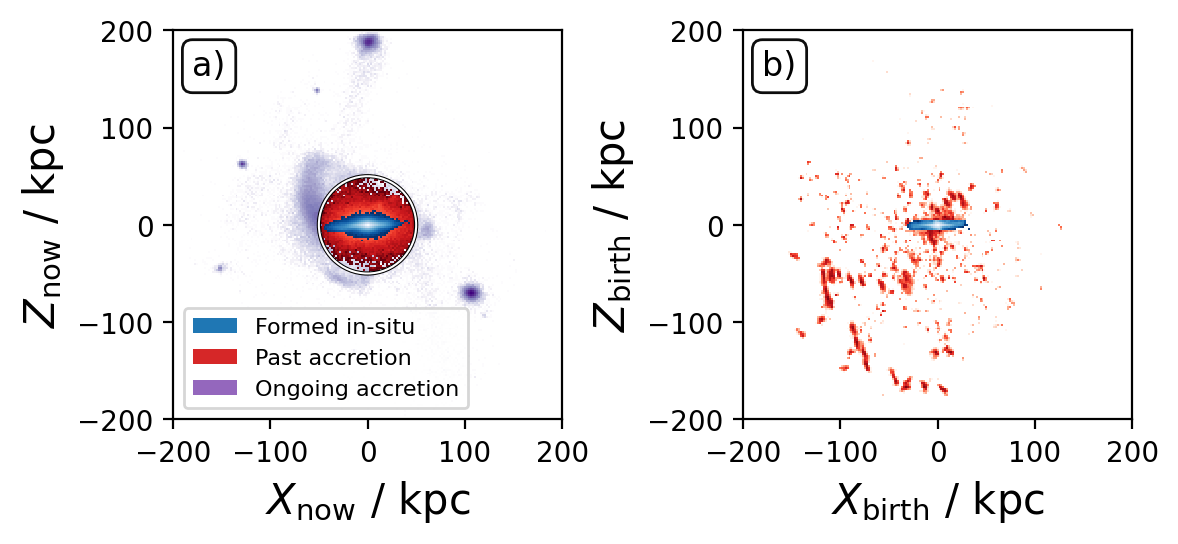
\includegraphics[width=\columnwidth]{figures/tracing_insitu_accretion_2.png}
    \caption{Tracing in-situ stars (blue) alongside past (red) and ongoing (purple) accretion components, shown in their present-day (panel~a) and birth (panel~b) positions at 100 Myr intervals. The red overdensities in panel b primarily reflect the same accreted galaxy observed at different epochs \href{https://github.com/svenbuder/gse_nihaouhd/tree/main/figures}{\faGithub}.}
    \label{fig:tracing_insitu_accretion_2}
\end{figure}

\subsection{A NIHAO-UHD Milky Way analogue simulation} \label{sec:data_simulation}

The simulation was performed using the smoothed particle hydrodynamics code \texttt{Gasoline2} \citep{Wadsley2017}, incorporating sub-grid turbulent diffusion, and adopting cosmological parameters from \citet{Planck2014}. The simulation setup and feedback mechanisms follow the NIHAO framework \citep{Wang2015}, with the zoom-in configuration and baryonic physics described in \citet{Buck2021}. Star formation and stellar feedback prescriptions follow \citet{Stinson2006} and \citet{Stinson2013}, respectively. Notably, the simulation used here is a more recent, higher-resolution rerun of the model in \citet{Buder2024}, and includes updated nucleosynthetic yields.

We focus our analysis on the main halo by identifying it with the Amiga Halo Finder \citep{Knollman2009}, using the build-tin tools of the \textsc{pynbody} package \citep{pynbody}. To orient the system, we rotate it face-on by aligning the angular momentum vector via \textsc{pynbody.analysis.angmom.faceon}. The simulated disk galaxy with spiral arms has a virial radius of $R\_{200} = 206\,\mathrm{kpc}$ and a total mass (baryons + dark matter) within this radius of $9.1 \times 10^{11}\,\mathrm{M_\odot}$. At present-day ($z = 0$), this includes $8.2 \times 10^{11}\,\mathrm{M_\odot}$ in dark matter, $6.4 \times 10^{10}\,\mathrm{M_\odot}$ in gas, and $2.3 \times 10^{10}\,\mathrm{M_\odot}$ in stars. The stellar mass resolution is approximately $7.5 \times 10^3\,\mathrm{M_{\odot}}$ per particle. For this study, we will refer to the galactocentric radius as the three-dimensional spherical radius
\begin{equation}
    R_{\mathrm{3D}} = \sqrt{x^2 + y^2 + z^2},
\end{equation}
rather than the cylindrical one, which is often used when focusing on studies of galactic discs \citep[for example by][for the same simulation]{Buder2025}.

\begin{figure}
    \centering
    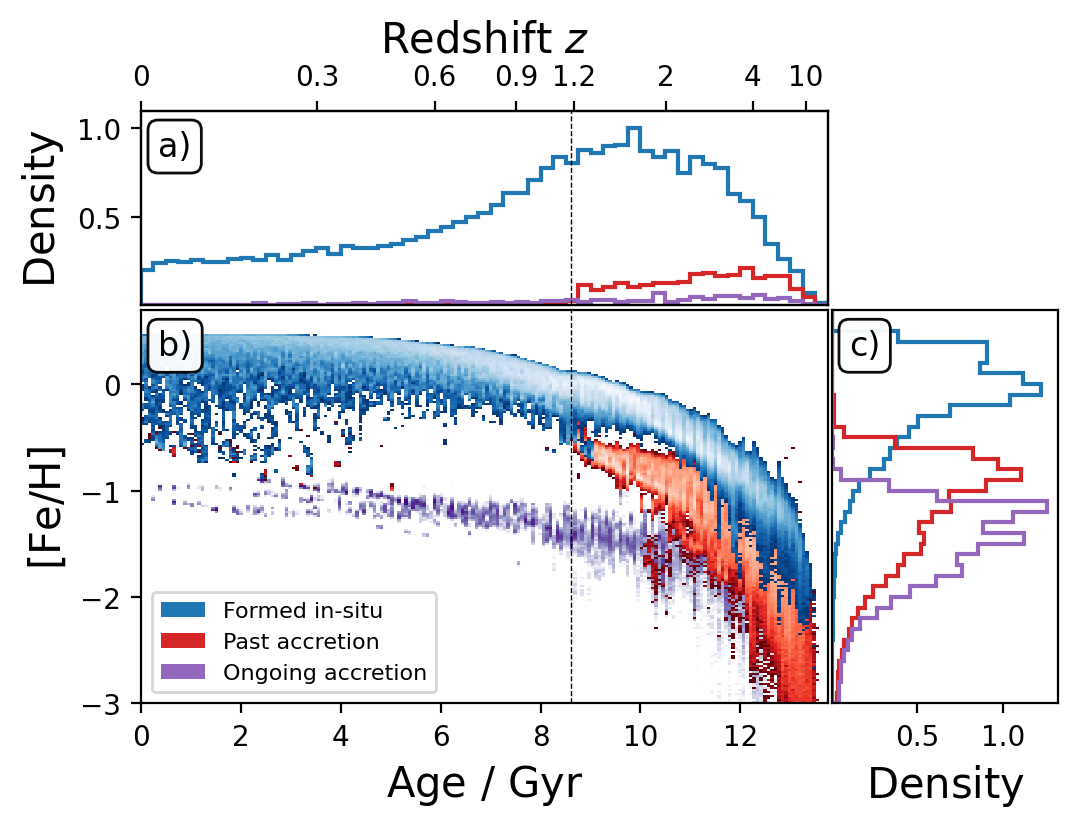
\includegraphics[width=\columnwidth]{figures/tracing_insitu_accretion_3.png}
    \caption{Age–metallicity distributions of in-situ (blue), previously accreted (red), and currently accreting (purple) stars, also shown as marginal 2D histograms with age (top) and [Fe/H] (right). A vertical dashed line indicates the time of the major merger around $8.6\,\mathrm{Gyr}$ ago \href{https://github.com/svenbuder/gse_nihaouhd/tree/main/figures}{\faGithub}.}
    \label{fig:tracing_insitu_accretion_3}
\end{figure}

Due to computational constraints, stars in the simulation are represented by tracer particles corresponding to simple stellar populations of uniform age, metallicity, and initial mass function (IMF). Chemical enrichment is computed using the \textsc{Chempy} framework \citep{Rybizki2017}, implemented by \citet{Buck2021}. We adopt the \texttt{alt} configuration, assuming a \citet{Chabrier2003} IMF with a high-mass slope of $\alpha_\text{IMF} = -2.3$ , spanning stellar masses from 0.1 to $100\,\mathrm{M_\odot}$, and covering metallicities $Z/Z_\odot \in [10^{-5},2]$. The enrichment includes contributions from asymptotic giant branch (AGB) stars, core-collapse supernovae (CCSN; $8 - 40\,\mathrm{M_\odot}$), and Type Ia supernovae (SNIa), modelled with an exponential delay-time distribution (slope $-1.12$), a minimum delay of $40\,\mathrm{Myr}$, and a normalised rate of $log_{10}(N_\mathrm{Ia}) = -2.9$. Yields are taken from \citet[][CCSN]{Chieffi2004}, \citet[][SNIa]{Seitenzahl2013}, and \citet[][AGB; \texttt{new\_fid} yields in \citealt{Buck2021}]{Karakas2016}, but no additional contributions, for example from neutron star mergers, for the rapid neutron-capture process. The simulation tracks elemental abundances for H, He, C, N, O, Ne, Mg, Al, Si, P, S, V, Cr, Mn, Fe, Co, and Ba on a Solar abundance scale by \citet{Asplund2009}. In alignment with the approach in \citet{Buder2025} and differing from \citet{Buder2024}, we adopt the simulated abundances directly, without applying empirical offsets. We note, however, that the median $\mathrm{[Fe/H]}$ for stars within a Solar-like galactocentric cylindrical radius of $R_\mathrm{GC} = \sqrt{x^2+y^2} = 8.2 \pm 0.5\,\mathrm{kpc}$ \citep{BlandHawthorn_Gerhard2016} and Solar-like age of $4.5 \pm 0.5\,\mathrm{Gyr}$ \citep{Soderblom2010} is $+0.15\,\mathrm{dex}$ and thus slightly enhanced with respect to the actual Milky Way. The star formation history, approximated by the stellar age histogram in Fig.~\ref{fig:tracing_insitu_accretion_3}a, of our analogue and Milky Way estimates \citep{Snaith2015} is qualitatively similar with steep rise from high redshifts to cosmic noon and a decreasing star formation thereafter. However, both quantitative differences as well as our chosen yields and other chemical evolution parameters can explain the offsets in abundances \citep[see also][]{Buck2021}.

\subsection{Tracing birth positions for stars of the main galaxy body}  \label{sec:data_birth_positions}

In a post-processing step, we have selected all star particles within a radius of $50\,\mathrm{kpc}$ from the present-day centre of mass of the simulation box. We have then gone back in simulation snapshot steps of $100\,\mathrm{Myr}$ and identified all star particles that were born between each time step. We then logged the positions of these star particles relative to the centre of mass of the main halo at the time, effectively tracing the birth positions with respect to the main halo.

\begin{equation}
    R_{\mathrm{birth}, \mathrm{3D}} = \sqrt{x_{\mathrm{birth}}^2 + y_{\mathrm{birth}}^2 + z_{\mathrm{birth}}^2}
\end{equation}

\subsection{Orbital properties}  \label{sec:data_orbit_properties}

The simulation is tracing information on both the Cartesian velocities of each particle $v_x, v_y, v_z$ as well as the potential $\phi$ at its current position\footnote{This simulation output is \texttt{potential\_phi} in the simulation FITS file.}. This allows us to calculate the specific Newtonian energy $E$ of the particle (per unit mass) as
\begin{align}
    E = \frac{1}{2}\left( v_x^2 + v_y^2 + v_z^2 \right) + \phi(R_\mathrm{3D})
\end{align}

In addition to the orbit energy, we also calculate orbit actions $J_{i \in [R, \varphi,z]}$ as integrals of motion with the \textsc{agama} package \citep{Vasiliev2019b}. We use \textsc{agama.Potential} to create a multipole expansion of the simulation potential by superimposing the dark matter, star, and gas particles (all weighted by their masses). This composite potential is passed to the \textsc{agama.ActionFinder}, which computes the approximate orbital actions ($J_R$, $J_\varphi \equiv L_Z$, and $J_Z$) for any given phase-space point (or in our case star particle) using the fast but approximating Stäckel fudge method \citep{Binney2012, Sanders2015b}.

%%%%%%%%%%%%%%%%%%%%%%%%%%%%%%%%%%%%%%%%%%%%%%%%%
%%%%%%%%%%%%%%%%%%%%%%%%%%%%%%%%%%%%%%%%%%%%%%%%%
\section{Analysis} \label{sec:analysis}

The ability to trace stellar birth positions in the NIHAO-UHD Milky Way analogue provides a unique opportunity to evaluate how much chemodynamical information is retained after a major merger. We begin by establishing a broad classification of stars into in-situ, past accretion, and ongoing accretion categories (Section~\ref{sec:analysis_broad_selection}). In Section~\ref{sec:analysis_dynamic_properties}, we examine the orbital properties of stars and quantify the efficiency of recovering accreted populations in integrals-of-motion space. Section~\ref{sec:analysis_chemodynamic_memory} then addresses how well the galaxy preserves its memory of stellar birth positions and chemical evolution in phase-space. Together, these analyses reveal how selection effects shape our ability to reconstruct the progenitor and chemical history of the last major merger.

\begin{figure*}
    \centering
    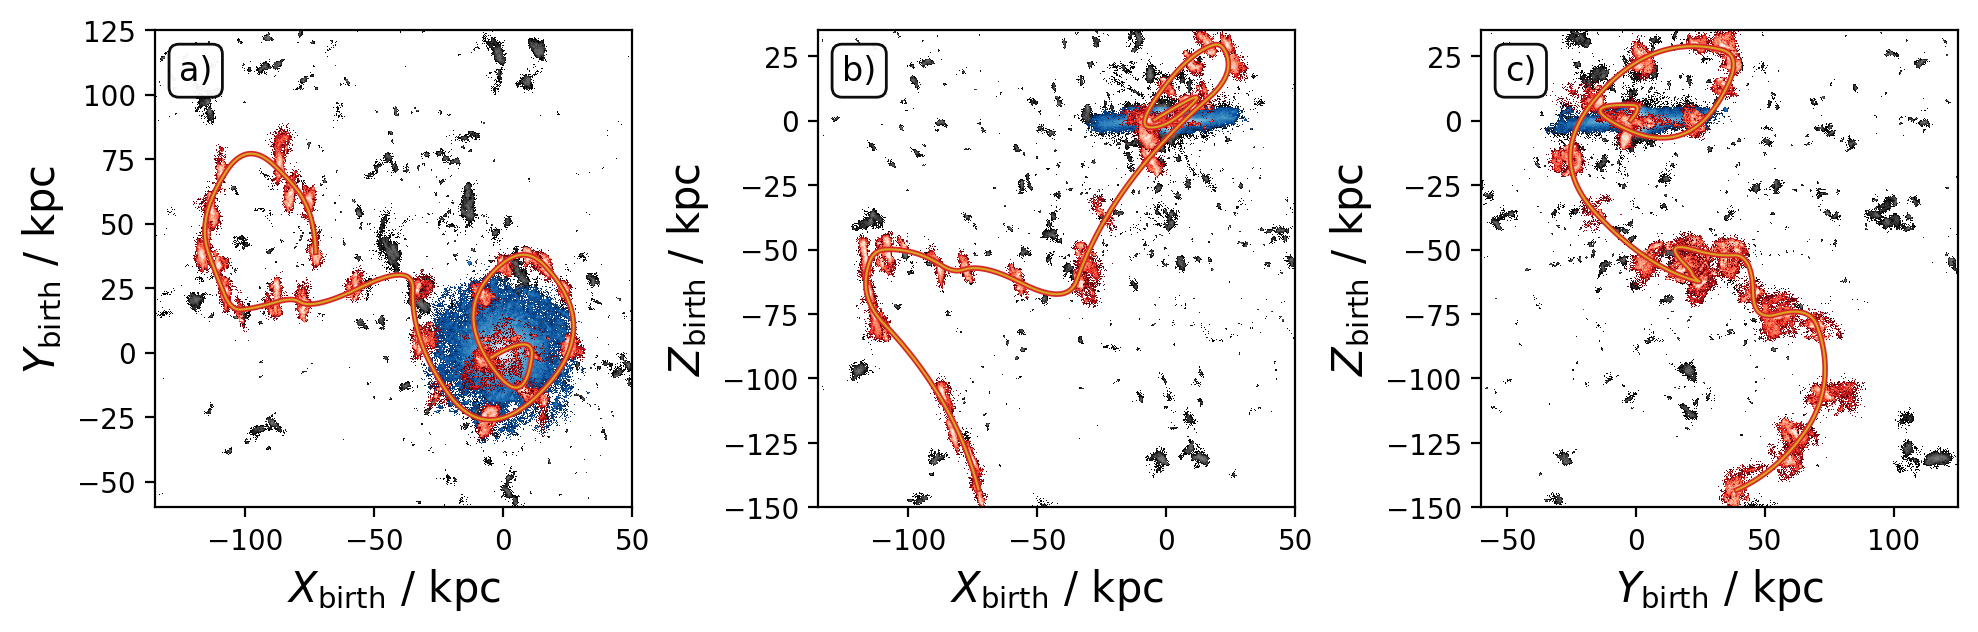
\includegraphics[width=\textwidth]{figures/tracing_xyz_birth_3.png}
    \caption{Birth positions in different Galactocentric planes of all star particles that are now within $50\,\mathrm{kpc}$ (grey density scale), where those born in-situ are in blue and those of the last major merger in red. Birth positions are estimated in $100\,\mathrm{Myr}$ steps and thus allow us to follow the changing position of star formation of the now accreted galaxy with respect to the Milky Way analogue. A dark golden line then interpolates the path of the now accreted galaxy \href{https://github.com/svenbuder/gse_nihaouhd/tree/main/figures}{\faGithub}.}
    \label{fig:tracing_xyz_birth_3}
\end{figure*}

%%%%%%%%%%%%%%%%%%%%%%%%%%%%%%%%%%%%%%%%%%%%%%%%%
\subsection{Tracing in-situ formation, past accretion, and ongoing accretion} \label{sec:analysis_broad_selection}

To broadly separate stars by their origin, we adopt a three-part classification: \textit{in-situ formation}, \textit{past accretion}, and \textit{ongoing accretion}. The goal is to construct a simple, interpretable, but still somewhat physically motivated scheme that captures the dominant contributors in each category without invoking overly complex selection criteria. Our classification is thus informed by both the present-day and birth positions of stars in the simulation (Fig.~\ref{fig:tracing_insitu_accretion_2}) as well as their age-metallicity distribution (Fig.~\ref{fig:tracing_insitu_accretion_3}). Based on these diagnostics, we define the following three selections.

Stars associated with the infalling dwarf galaxies with lower [Fe/H], selected as part of the sample with
\begin{equation}
\text{Ongoing accretion:} \qquad
\begin{cases}
&R_\mathrm{3D} > 50\,\mathrm{kpc} \text{ or }\\
&E > 0\,\mathrm{kpc\,km\,s^{-1}} \text{ or } \\
&( \mathrm{age} < 10\,\mathrm{Gyr} \text{ and }  [\mathrm{Fe}/\mathrm{H}] < -1 )
\end{cases}
\end{equation}
The last adjustment is included to identify the full extend of younger stars of the clearly separated dwarf galaxies in Fig.~\ref{fig:tracing_insitu_accretion_2}b that are either already within $50\,\mathrm{kpc}$ or already have negative orbit energies.

Stars now within $50\,\mathrm{kpc}$ but with signs of external origin at birth are defined as
\begin{equation} \label{eq:selection_past_accretion}
    \text{Past accretion:} \qquad \begin{cases}
    R_{\mathrm{3D}} \leq 50\,\mathrm{kpc} \text{ and }\\
    E < 0\,\mathrm{kpc\,km\,s^{-1}} \text{ and } \\
    ( R_{\mathrm{birth}, \mathrm{3D}} > 50\,\mathrm{kpc} \text{ or } |z_{\mathrm{birth}}| > 5\,\mathrm{kpc} )
    \end{cases}
\end{equation}
In particular the selection of stars with $|z_{\mathrm{birth}}| > 5\,\mathrm{kpc}$ is an important and clean adjustment, as it adds the $28\,\%$ of finally selected stars that were born in the last stages of the inclined merger. We have optimised this this selection via the position of selected stars in the age-metallicity plane of Fig.~\ref{fig:tracing_insitu_accretion_2}b.

All remaining stars formed and residing within the central region were defined as
\begin{equation} \label{eq:selection_insitu}
\text{In-Situ:} \qquad
\begin{cases} 
    R_{\mathrm{3D}} \leq 50\,\mathrm{kpc} \text{ and }\\
    E < 0\,\mathrm{kpc\,km\,s^{-1}} \text{ and } \\
    R_{\mathrm{birth}, \mathrm{3D}} \leq 50\,\mathrm{kpc} \text{ and }\\
    |z_{\mathrm{birth}}| \leq 5\,\mathrm{kpc}
\end{cases}
\end{equation}

While our selection is certainly not perfect, it provides a reasonable compromise. Each of the three groups is dominated by stars that plausibly reflect their intended origin, with minimal overlap. 95\% of the stars selected as currently being accreted are unbound, that is, have positive specific orbit energies. Similarly, 99\% of stars selected as accreted in the past are currently on bound orbits with negative specific orbit energies. Tracing the star formation in Figs.~\ref{fig:tracing_insitu_accretion_2} and \ref{fig:tracing_insitu_accretion_3}, only 6771 star particles ($2.7\,\%$ of accreted sample) fall into a hard-to-classify category of overlapping chemistry ($-0.6 < \mathrm{[Fe/H]} < -0.2$) and birth positions between the last stage of the merger around $8.50$ and $8.65\,\mathrm{Gyr}$ ago. Our selection thus provides a useful basis for subsequent analysis.

Of the $2.9 \times 10^6$ star particles ($2.3 \times 10^{10}\,\mathrm{M_\odot}$), we select $87.9\,\mathrm{\%}$ ($2.0 \times 10^{10}\,\mathrm{M_\odot}$) as in-situ, $8.5\,\mathrm{\%}$ ($1.9 \times 10^{9}\,\mathrm{M_\odot}$) as previously accreted and $3.5\,\mathrm{\%}$ ($8.1 \times 10^{8}\,\mathrm{M_\odot}$) as currently being accreted. At present-day the stellar mass ratio of previously accreted galaxy compared to the Milky Way analogue is 1:11. When only counting stars with ages above $8.6\,\mathrm{Gyr}$ ago, that is older than the merger, the mass ratio is 1:5 ($1.9 \times 10^{9}\,\mathrm{M_\odot}$ vs. $9.6 \times 10^{9}\,\mathrm{M_\odot}$).

While versions of Figs.~\ref{fig:tracing_insitu_accretion_2}a and \ref{fig:tracing_insitu_accretion_3} have already been analysed for a lower resolution version of this simulation by \citet{Buder2024}, the pattern of birth positions in Fig.~\ref{fig:tracing_insitu_accretion_2}b is intriguing, as we can see several overdensities that follow each other like a string of pearls.
For each of these pearls, representative of star formation within $100\,\mathrm{Myr}$ post-processing steps (see Sec.~\ref{sec:data_birth_positions}), we identify a spatial region within a reasonable age interval (see Tab.~\ref{tab:birth_position_tabular}) that traces the median birth position and then fit and interpolate a smooth function\footnote{We use \textsc{scipy.interpolate}'s \textsc{splprep} and \textsc{splev} functions \citep{Scipy} to fit and then evaluate a 2-degree B-spline function with smoothing value 100.} to the discrete positions.  We visualise this in Fig.~\ref{fig:tracing_xyz_birth_3} as a golden thread that reliably\footnote{Due to the unstable orientation of the main galaxy for snapshots more than $12\,\mathrm{Gyr}$ ago, this reference frame is only reliable to trace the major merger galaxy (visible as several of the grey overdensities in Fig.~\ref{fig:tracing_xyz_birth_3}) after the main galaxy's orientation stabilised.} traces the path of merged galaxy based on the star formation from $12\,\mathrm{Gyr}$ ago until its last star formation period during the merger with the analogue around $8.6\,\mathrm{Gyr}$ ago. While not the focus of our work, we note that the galaxy that later merged with the Milky Way encountered a merger of its own with another galaxy $10.8\,\mathrm{Gyr}$ ago around $(X_\mathrm{birth},Y_\mathrm{birth},Z_\mathrm{birth}) = (-120,25,-55)\,\mathrm{kpc}$ that changed its course. In almost all cases, we see the now accreted galaxy as disk galaxy, most clearly in the almost face-on few of the galaxy across the time steps of Fig.~\ref{fig:tracing_xyz_birth_3}c.

We will investigate how birth positions may be related to present-day properties in Sec.~\ref{sec:analysis_chemodynamic_memory}. But first, we provide an overview of orbit properties in the simulated galaxy. %This will set us up for analysing our first objective of analysing how similar the present-day orbital distribution of accreted stars in the NIHAO-UHD Milky Way analogue are to those found by \citet{Mori2024} and explored observationally in \citet{Skuladottir2025}.

%%%%%%%%%%%%%%%%%%%%%%%%%%%%%%%%%%%%%%%%%%%%%%%%%
\subsection{Dynamic properties and selection efficiency of accreted stars via integrals of motions} \label{sec:analysis_dynamic_properties}
%What can we learn about the selection efficiency of accreted stars in integrals of motions space \citep{Helmi2018, Feuillet2021, Buder2022, Monty2024}?

As customary in recent observational Galactic dynamical studies \citep[for example][]{Helmi2018, Trick2019, Helmi2020, Buder2022}, we take a look at the distribution of stars in two of the integrals of motion, namely orbit energy $E$ over angular momentum $L_Z$ (top rows of Fig.~\ref{fig:lz_e_jr}) or a condensed version with radial action $J_R$ of angular momentum $L_Z$ (bottom rows of Fig.~\ref{fig:lz_e_jr} using $\sqrt{J_R}$).

\begin{figure*}
    \centering
    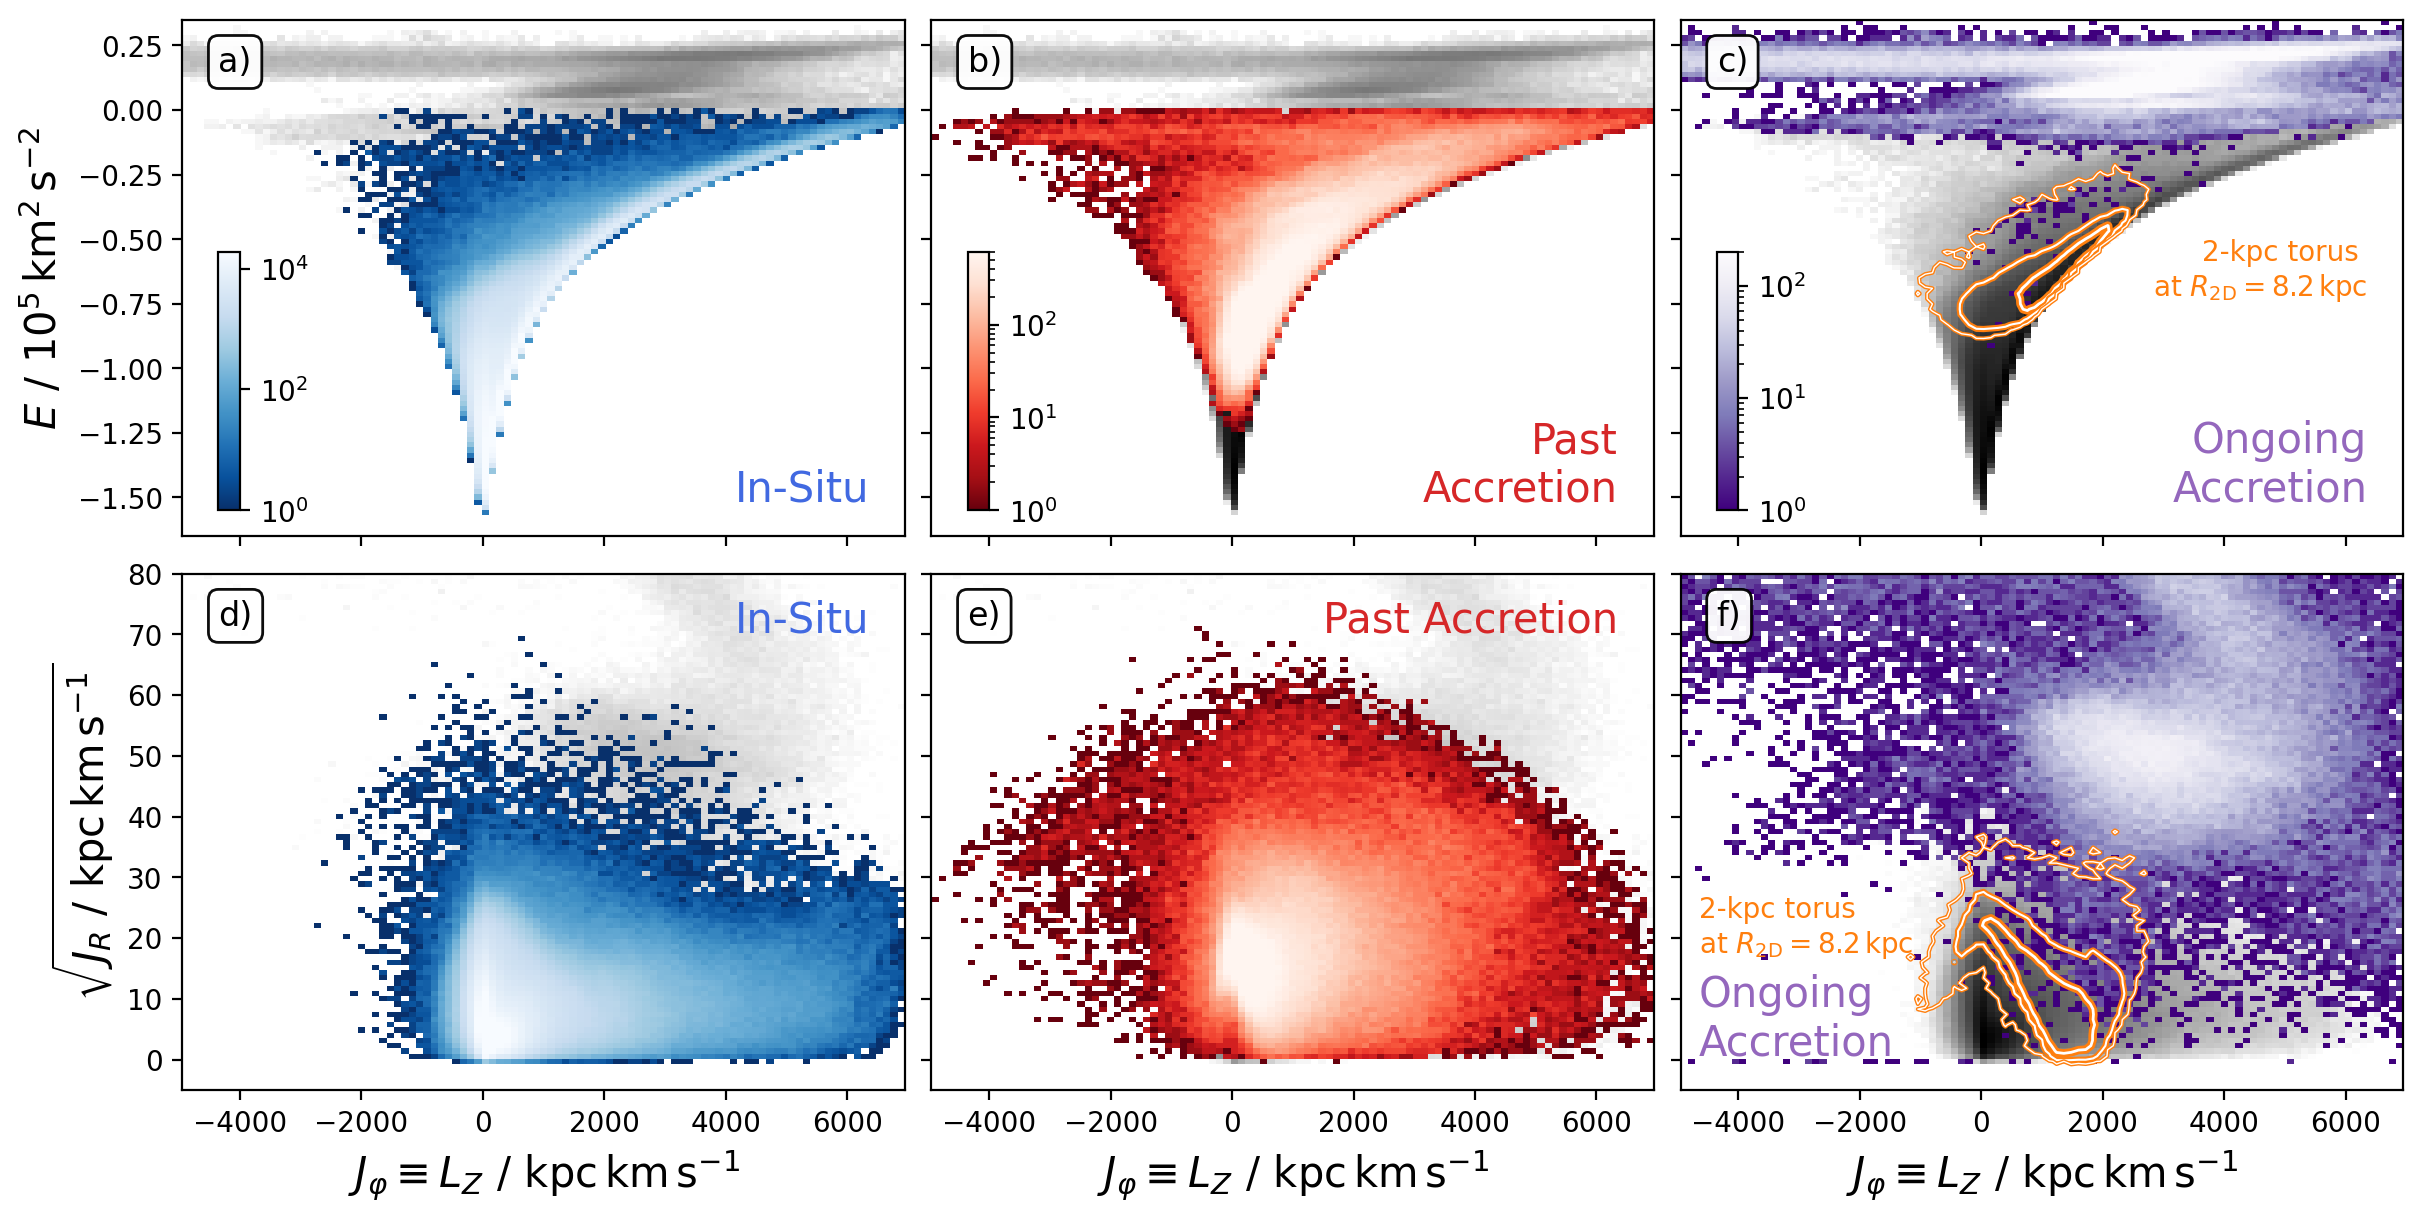
\includegraphics[width=\textwidth]{figures/lz_e_jr.png}
    \caption{Orbit properties of in-situ formed stars (blue, left panels), past accretion (red, middle panels), and ongoing accretion (purple, right panels). Both the specific energy $E$ (upper panels) and the radial action $J_R$ (lower panels) are shown with the angular momentum $J_\varphi \equiv L_Z$. Stars undergoing accretion, currently located in the Solar-analogue neighbourhood of a 2\,kpc torus around $R_\mathrm{2D} = 8.2\,\mathrm{kpc}$, are indicated with orange density contours (the 68th, 95th, and 99.7th percentiles of stars) \href{https://github.com/svenbuder/gse_nihaouhd/tree/main/figures}{\faGithub}.
    \label{fig:lz_e_jr}}
\end{figure*}

Fig.~\ref{fig:lz_e_jr}a shows that most of the in-situ stars of the spiral galaxy are moving on circular disc orbits as they are concentrated along a curved ridge tracing the maximum angular momentum allowed at each energy. In Fig.~\ref{fig:lz_e_jr}d, these stars show low radial actions of $J_R < 10^2\,\mathrm{kpc\,km\,s^{-1}}$. In both figures, we note a broader excess of stars with higher (less negative) orbit energies ($E > -10^5\,\mathrm{km^2\,s^{-2}}$) and larger radial actions ($J_R \gtrsim 10^2\,\mathrm{kpc\,km\,s^{-1}}$) in the area of negligible net rotation ($L_Z \sim 0\,\mathrm{kpc\,km\,s^{-1}}$). This region of dynamically hotter stars with more (radially) eccentric orbits is also densely populated by stars that have been accreted previously (see Figs.~\ref{fig:lz_e_jr}b and \ref{fig:lz_e_jr}e around $L_Z \sim 0\,\mathrm{kpc\,km\,s^{-1}}$). The orbits of previously accreted stars extend from these regions of low absolute angular momentum $\vert L_Z\vert$ towards similar positive angular momenta, but show typically higher (less bound) orbit energies and larger radial actions, typical for more radial and eccentric orbits. Stars associated with ongoing accretion (Figs.~\ref{fig:lz_e_jr}c, \ref{fig:lz_e_jr}f), trace partially phase-mixed tidal debris from currently disrupting satellites as well as surviving satellites. They exhibit a wide range in angular momentum, often with retrograde orbits, and occur at high, predominantly positive energies.

As we show the whole galaxy in these figures, we note that the distributions in Fig.~\ref{fig:lz_e_jr} look different from what has been found observationally in the Milky Way's Solar neighbourhood \citep[see for example][]{Helmi2018,Trick2019,Das2020,Buder2022}. We have included orange contours in Figs.~\ref{fig:lz_e_jr}c and \ref{fig:lz_e_jr}f which trace the 68th, 95th, and 99.7th percentiles of stars in a torus with a tube radius of $2\,\mathrm{kpc}$ at a galactocentric cylindrical distance of $R_\mathrm{2D} = 8.2\,\mathrm{kpc}$, typical of footprints of current Milky Way surveys \citep[for example][]{SDSSDR17, Katz2023, Buder2025}. These are distributed mainly within angular momenta of $0 < L_Z~/~\mathrm{kpc\,km\,s^{-1}} < 2000$ and show circular orbits (low $J_R$) at their largest angular momenta and more eccentric, radial orbits for stars with low absolute angular momenta.

In Fig.~\ref{fig:lz_e_jr}, we are especially intrigued by the extended distribution of accreted stars towards the lowest energies (Fig.~\ref{fig:lz_e_jr}b) and the significant overlap with the inner in-situ galaxy (Fig.~\ref{fig:lz_e_jr}a). These are regions that are not extensively explored by surveys of the Solar neighbourhood, but are expected to contain a significant fraction of accreted stars, well hidden within a labyrinth of in-situ stars. We have calculated the relative fraction of previously accreted stars to the main body of the galaxy ($R_\mathrm{3D} < 50\,\mathrm{kpc}$), in Fig.~\ref{fig:fraction_accreted_in_situ_lz}. Overall, we see that in-situ stars dominate (blue regions) for specific energies below $E < -0.58\times10^{5}\,\mathrm{kpc\,km\,s^{-1}}$ as well as radial actions below $J_R < 20^2\,\mathrm{kpc\,km\,s^{-1}}$ and in general stars on circular orbits, with the latter being situated along the righter edge of distribution. Accreted stars dominate (red regions) in the less bound and non-circular regions of the diagrams.

\begin{figure}
    \centering
    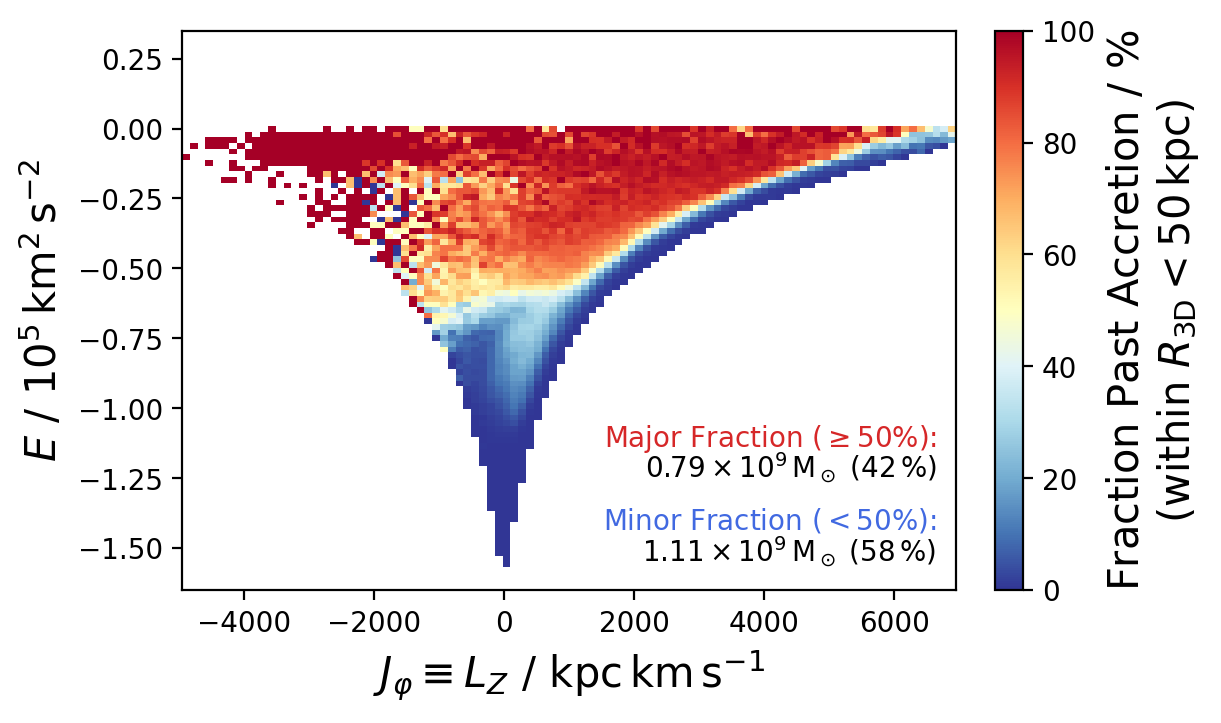
\includegraphics[width=\linewidth]{figures/fraction_accreted_in_situ_lz_e.png}
    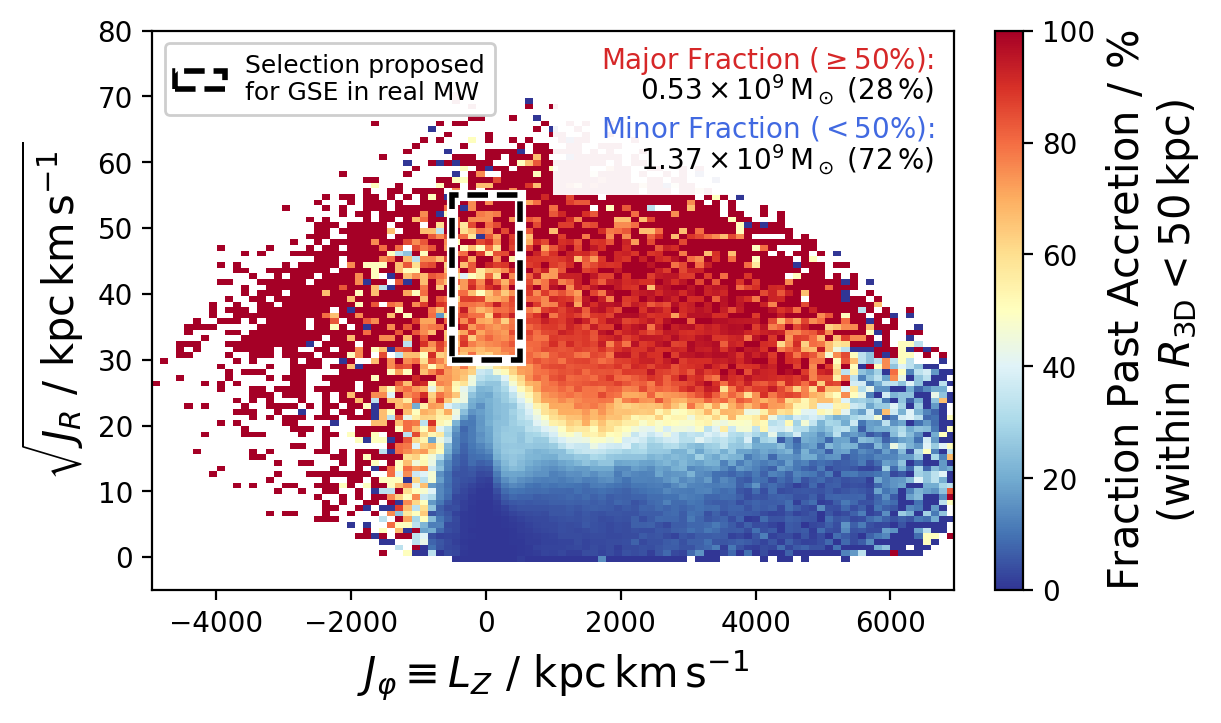
\includegraphics[width=\linewidth]{figures/fraction_accreted_in_situ_lz_jr.png}
    \caption{Angular momentum $J_\varphi \equiv L_Z$ vs. Specific energy $E$ (top panel) and radial action $J_R$ for stars (bottom panel) for stars within $R_\mathrm{3D} < 50\,\mathrm{kpc}$ at redshift $z=0$. Bins are coloured by the fraction of previously accreted stars (defined as Figs.~\ref{fig:lz_e_jr}b/(a+b) and \ref{fig:lz_e_jr}d/(d+e), respectively). We have added the selection proposed by \citet{Feuillet2020} for the real Milky Way as dashed black box. For a figure that includes ongoing accretion ($R_\mathrm{3D} > 50\,\mathrm{kpc}$) in the denominator, see Fig.~\ref{fig:fraction_accreted_in_situ_lz_total}~\href{https://github.com/svenbuder/gse_nihaouhd/tree/main/figures}{\faGithub}.}
    \label{fig:fraction_accreted_in_situ_lz}
\end{figure}

We note the remarkable similarity between Fig.~\ref{fig:fraction_accreted_in_situ_lz} and those presented by \citet[][their Fig.~1]{Belokurov2022} and \citet[][their Fig.~1]{Monty2024} who plot the same plot of angular momentum $J_\varphi = L_Z$ vs. specific energy $E$, but colour-coded by [Al/Fe] and [Eu/Si], respectively. The latter work found a significant change in the median chemical compositions around 50\% of the lowest orbit energies for their chosen potentials\footnote{The different amplitudes of the orbit energies that mark the boundary between being dominated by accreted or in-situ populations of $-0.66 \times 10^5\,\mathrm{km^2\,s^{-2}}$ in our simulation compared to $-1.6 \times 10^5\,\mathrm{km^2\,s^{-2}}$ by \citet{Monty2024} or $-0.75 \times 10^5\,\mathrm{km^2\,s^{-2}}$ by \citet{Belokurov2022} can be explained by both the different actual galaxies and potentials.} and attribute them to a transition of accreted to in-situ stars. We find a similar trend of significantly changing the dominant population from accreted to in-situ stars at about 50\,\% of the lowest orbital energy of the sample. As previously noted, we find that almost half the population of accreted stars is hidden in the region of $E < -0.58\times10^5\,\mathrm{km^2\,s^{-2}}$ that is dominated by in-situ stars. However, when selecting only from the regions in the $L_Z$-$E$ diagram with a fraction of past accretion larger than $50\mathrm{\%}$ (orange-red regions in Fig.~\ref{fig:fraction_accreted_in_situ_lz}), we only select $42\,\mathrm{\%}$% of stars of the last major merger.

For the simulated Milky Way analogue, we find that the accreted stars dominate in regions of more radial orbits, typically with $J_R > 20^2\,\mathrm{kpc\,km\,s^{-1}}$ and slightly higher values of $J_R > 30^2\,\mathrm{kpc\,km\,s^{-1}}$ for the region of $\vert L_Z \vert \lesssim 1000\,\mathrm{kpc\,km\,s^{-1}}$. As we are plotting the whole galaxy in this figure, we include a significant amount of stars with high radial actions, which are typically not visiting the Solar neighbourhood \citep[compare Figs.~\ref{fig:lz_e_jr}e and \ref{fig:lz_e_jr}f and see for example][]{Feuillet2019}. A significant region of the action-action space in the Milky Way is populated by other accreted systems \citep[for example][]{Myeong2019, Naidu2020}. It is thus not surprising, that the often suggested regions to cleanly select the stars of the last major merger in the Milky Way have been restricted to a small window around $\vert L_Z \vert < 500\,\mathrm{kpc\,km\,s^{-1}}$ and $30^2 < J_R~/~\mathrm{kpc\,km\,s^{-1}} < 55$ \citep{Feuillet2021, Buder2022}, which we have added to Fig.~\ref{fig:fraction_accreted_in_situ_lz}b for reference. Interestingly, our simulation indicates that the suggested lower limit in radial actions coincides with the region where the ratio of accreted to in-situ stars shifts. Contamination thus rapidly increases when accreted stars are selected solely by low radial actions in action space. While \citet{Buder2022} found that only $29 \pm 1\,\mathrm{\%}$ of chemically identifiable accreted stars in their sample are within this clean dynamical selection box. Similarly, we find that a restricted selection from Fig.~\ref{fig:fraction_accreted_in_situ_lz} in regions where accreted stars dominate only selects $28\,\mathrm{\%}$% of all accreted stars \citep[for a study of other selection criteria and their purity as well as completeness see][]{Carrillo2024}.

For completeness, we have also calculated the percentage ratio of previously accreted stars to all stars in each of the $L_Z$-$E$ and $L_Z$-$\sqrt{J_R}$ bins. We append them to this paper in Fig.~\ref{fig:fraction_accreted_in_situ_lz_total} to visualise the relatively minor contaminating effect of ongoing accretion at higher energies, similar to that of the Sagittarius dwarf spheroidal galaxy in the Milky Way. However, the overall estimate of selecting accreted stars from dominant regions does not shift significantly, that is, only from $42\,\mathrm{\%}$% to $41\,\mathrm{\%}$%. Similarly, including ongoing accretion to calculate the fraction in the $L_Z$ vs. $\sqrt{J_R}$ domain (compare Figs.~\ref{fig:fraction_accreted_in_situ_lz} and \ref{fig:fraction_accreted_in_situ_lz_total}a) insignificantly changed the selection ratio from $28\,\mathrm{\%}$% to $26\,\mathrm{\%}$%. As we are able to use the birth positions for a rather clean selection of in-situ and accreted stars, we can now turn to the analysis of the memory of the progenitor galaxy that might still be imprinted in the present-day properties of the accreted stars.

\begin{table}
    \centering
    \renewcommand{\arraystretch}{1.5}
    \caption{Energy selections of the four zones of previously accreted stars used in Sec.~\ref{sec:analysis_chemodynamic_memory} and the median [Fe/H] in each bin, with error bars as in Fig.~\ref{fig:fe_h_histograms}.}
    \begin{tabular}{cc} 
    \hline\hline
    Energy Selection & {[Fe/H]} \\
    \hline
    $ \qquad \quad ~~~\, E~/~\mathrm{kpc\,km\,s^{-1}}<-0.77$ & $-0.94_{-0.67}^{+0.28}$% \\
    $-0.77 \leq E~/~\mathrm{kpc\,km\,s^{-1}} < -0.58$ & $-1.01_{-0.63}^{+0.31}$% \\
    $-0.58 \leq E~/~\mathrm{kpc\,km\,s^{-1}} < -0.37$ & $-1.1_{-0.6}^{+0.4}$% \\
    $ -0.37 \leq  E~/~\mathrm{kpc\,km\,s^{-1}}\qquad \quad ~~~\,$ & $-1.4_{-0.6}^{+0.5}$% \\
    \hline
    All energies & $-1.1_{-0.7}^{+0.4}$% \\
    \hline\hline
    \end{tabular}
    \label{tab:energy_selection}
    % \renewcommand{\arraystretch}{1.0}
\end{table}

\begin{figure}
    \centering
    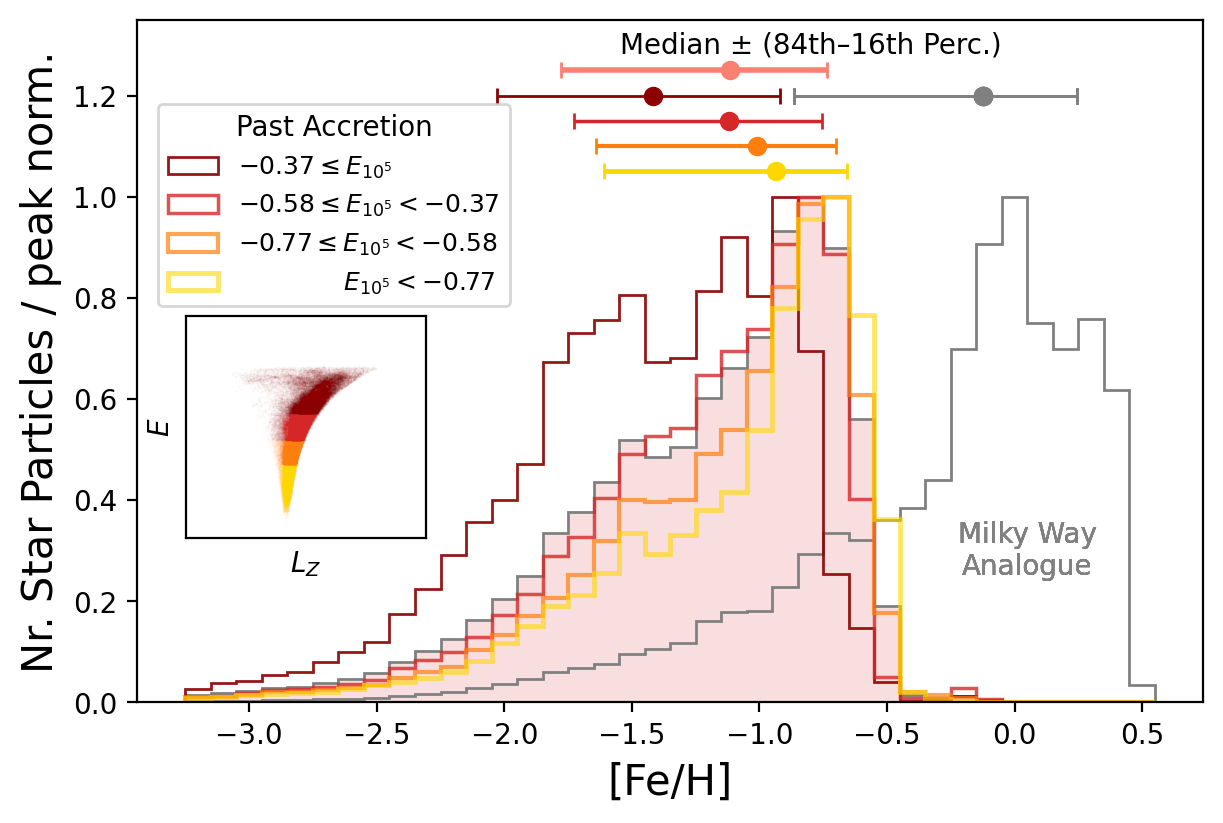
\includegraphics[width=\columnwidth]{figures/fe_h_histograms.png}
    \caption{Histograms of ${\mathrm{[Fe/H]}}$ distributions of the whole galaxy (grey), and its previously accreted stars with different orbit energies as given in Table \ref{tab:energy_selection} (more negative energies from red to yellow, as shown in the inset panel of $L_Z$ vs. $E$). The percentiles of each distribution are plotted at the top right of the figure and show an increase of average [Fe/H] with more negative energies. See \href{https://github.com/svenbuder/gse_nihaouhd/tree/main/figures}{\faGithub} for individual figures showing the build-up of this plot.}
    \label{fig:fe_h_histograms}
\end{figure}

%%%%%%%%%%%%%%%%%%%%%%%%%%%%%%%%%%%%%%%%%%%%%%%%%
\subsection{Dependence of the chemical and birth position on energy} \label{sec:analysis_chemodynamic_memory}
% What chemical and birth position memory of the progenitor galaxy is retained in integrals of motion space \citep{Skuladottir2025}?

After presenting an overview of the energies and actions of in-situ and, more importantly, accreted stars in the simulation, we focus on how the properties of accreted stars depend on orbital energy $E$. This question was already investigated by \citet{Skuladottir2025}, using a small sample of 33 accreted stars with high-quality chemical abundance measurements, which they divide into two samples of 20 and 13 stars with energies above or below $E = -0.45\times10^{5}\,\mathrm{kpc\,km\,s^{-1}}$, respectively. Our selection of accreted stars consists of a quarter of a million star particles, enabling us to dissect our simulated galaxy into more samples. We thus decide to divide the sample into quartiles, or `zones', of orbit energy, which we list in Table~\ref{tab:energy_selection} and visualise through the inset shown in Fig.~\ref{fig:fe_h_histograms}.

These four samples, selected to have roughly 25\% of accreted stars in each of them, now allow us to investigate the memory or different properties across different orbit energies. In particular, we are interested in the change of the (i)~overall metallicity [Fe/H], (ii)~chemical abundances, (iii)~present-day positions, and (iv)~birth positions, which we analyse separately below.

\begin{figure*}
    \centering
    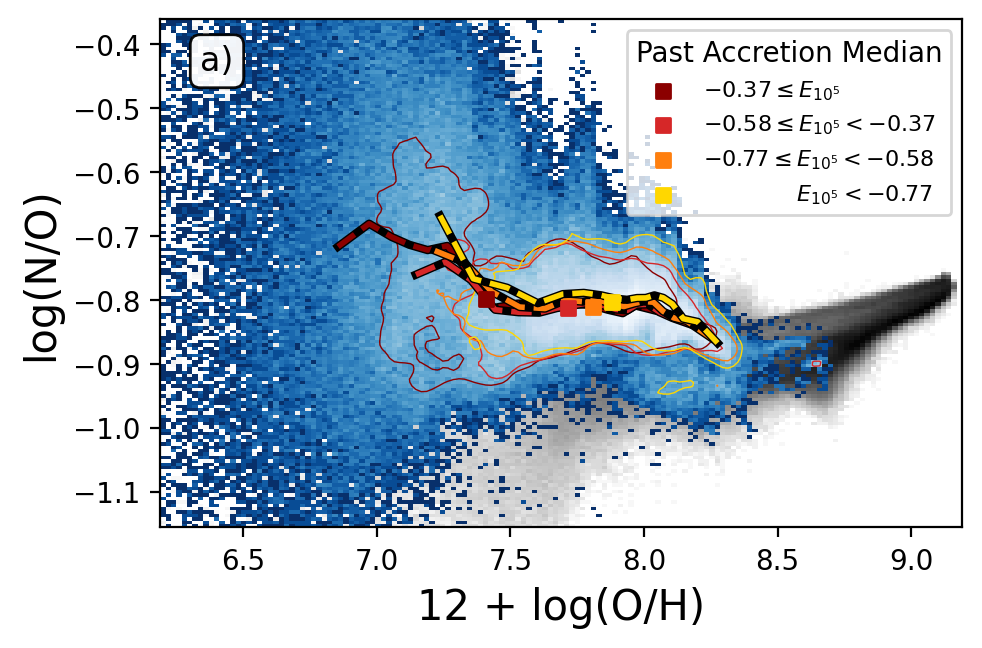
\includegraphics[width=0.33\textwidth]{figures/xfe_feh_zones_NO.png}    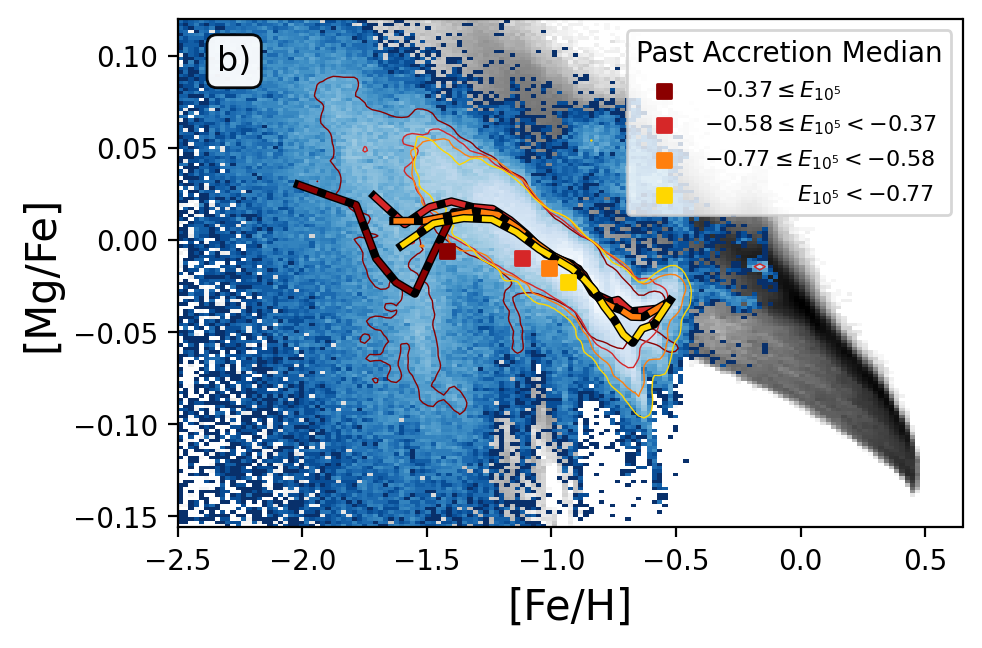
\includegraphics[width=0.33\textwidth]{figures/xfe_feh_zones_Mg.png}
    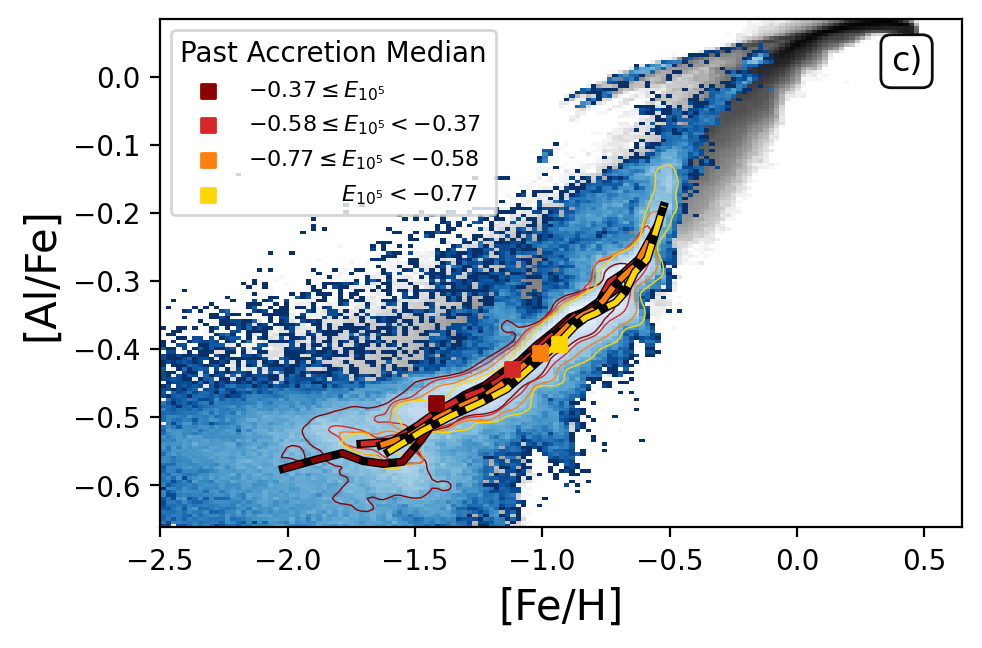
\includegraphics[width=0.33\textwidth]{figures/xfe_feh_zones_Al.png}
    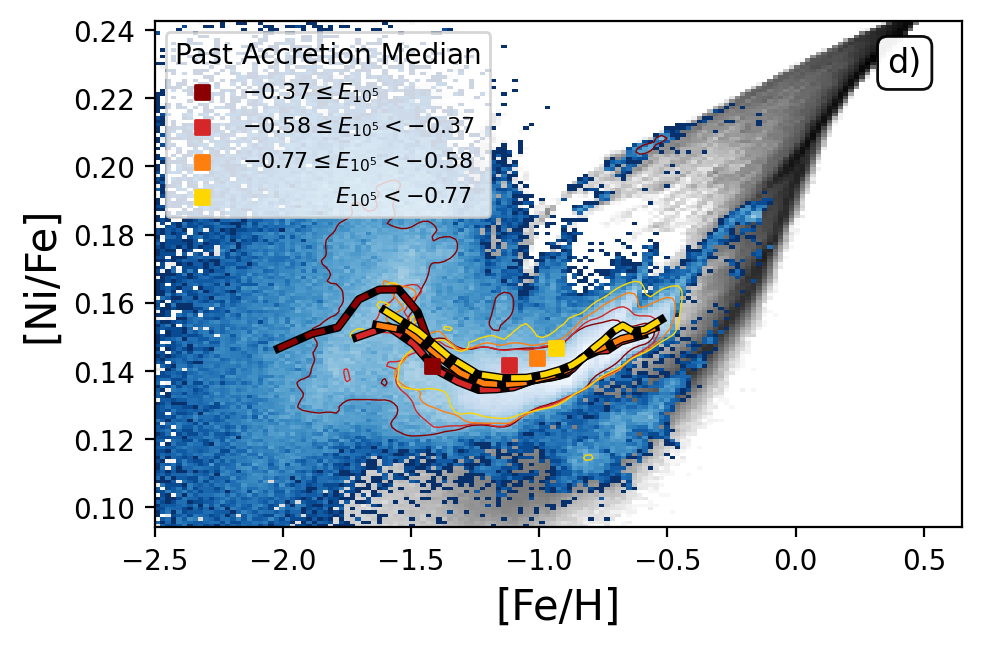
\includegraphics[width=0.33\textwidth]{figures/xfe_feh_zones_Ni.png}
    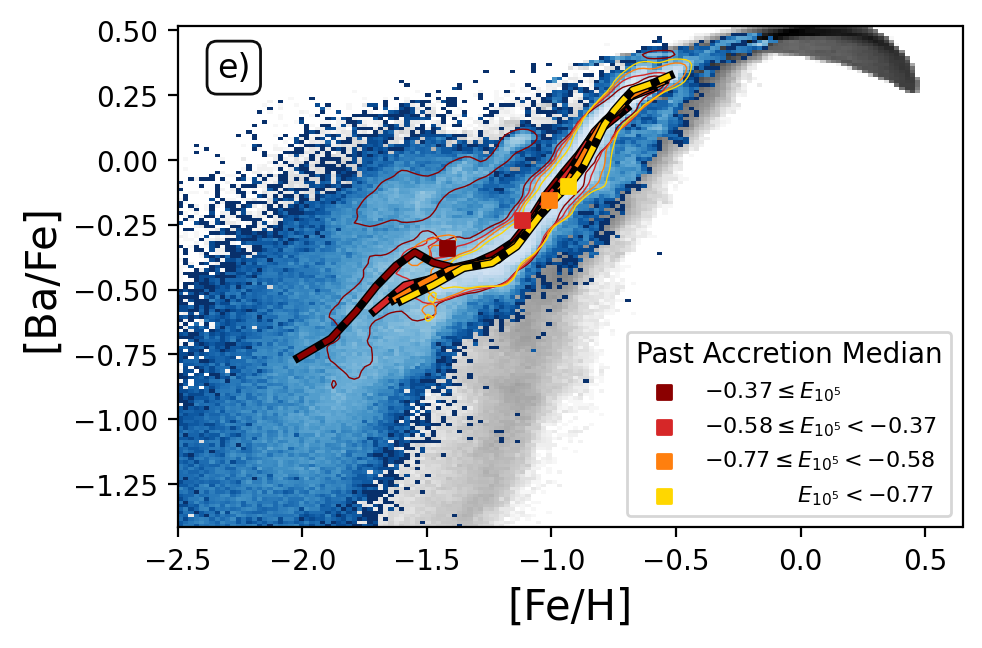
\includegraphics[width=0.33\textwidth]{figures/xfe_feh_zones_Ba.png}
    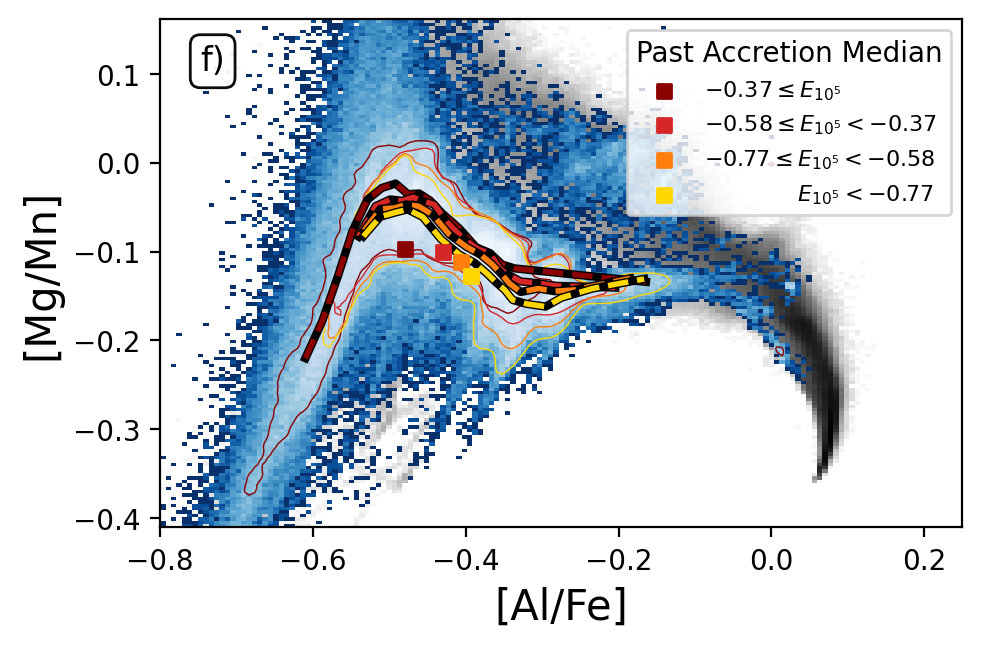
\includegraphics[width=0.33\textwidth]{figures/xfe_feh_zones_MgMn.png}
        \caption{Abundance distributions of (past) accreted stars in blue, while the whole simulation is shown in the background (black). Yellow, orange, light and dark red show the distribution contours of 68\% of accreted stars from the different energy quantiles (same as in Fig.~\ref{fig:fe_h_histograms}). Squares show the median abundances of each sample.}
    \label{fig:xfe_feh_zones}
\end{figure*}

\begin{figure*}
    \centering
    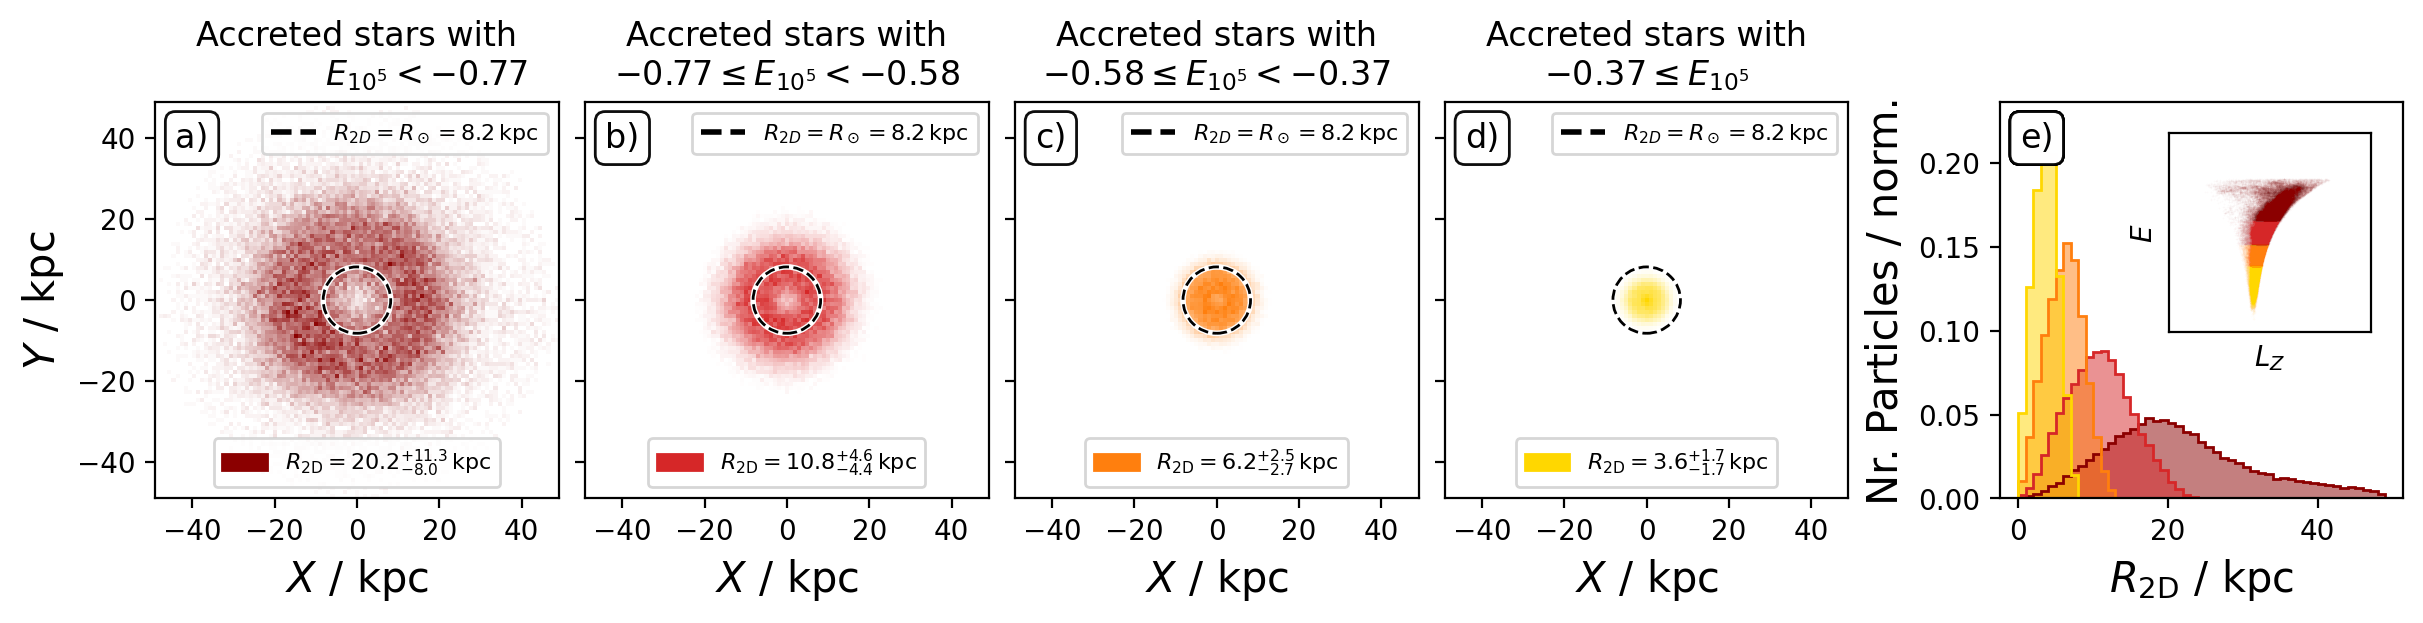
\includegraphics[width=\textwidth]{figures/xy_distribution_ezones.png}
    \caption{Present-day spatial distribution of accreted stars in the Galactocentric $X$-$Y$ plane. Panels a-d) show the density distribution of accreted stars with highest to lowest orbit energy quartiles, where the dashed circle shows a solar-analogue $R_\mathrm{2D}=8.2$\,kpc. Panel legends list the 50th and 16th-84th percentiles of galactocentric cylindrical radii $R_\mathrm{2D}$. Panel e) shows the $R_\mathrm{2D}$ distributions, with an inset visualising the $L_Z$ vs. $E$ selection. See Fig.~\ref{fig:xz_distribution_ezones} for a similar figure showing the $X$-$Z$ plane.}
    \label{fig:xy_distribution_ezones}
\end{figure*}

\subsubsection{Orbital memory of {[Fe/H]} abundance}

In Fig.~\ref{fig:fe_h_histograms}, we plot the histograms of iron abundance [Fe/H] for the different energy zones with different colours (yellow to dark red for increasing $E$) and the normalised histogram of all accreted stars as filled histogram in the background. The median values of accreted stars ($\mathrm{[Fe/H]} = $$-1.1_{-0.7}^{+0.4}$%) are 1\,dex than the in-situ galaxy, which has a median $\mathrm{[Fe/H]} = $$-0.1_{-0.5}^{+0.3}$%, where the errors are the 84-16th percentiles. This is consistent with expectations from the mass-metallicity relation \citep[for example][]{Gallazzi2005, Kirby2013} and the lower mass of the accreted system in comparison to the main galaxy (1:11).

For most distributions, we see asymmetric, negatively skewed distributions in logarithmic [Fe/H] abundance space, which could constitute a more normal distribution in linear $N_\mathrm{Fe}/N_\mathrm{H}$ number density space. Compared to the other zones, the highest orbit energies (dark red) shows a broader and double-peaked distribution. This region is particularly prone to contamination from the many smaller accretion events of metal-poor systems (visible as many smaller dots in Fig.~\ref{fig:tracing_insitu_accretion_2}b). When comparing our overall selection of accreted stars in this energy zone with those that follow the golden thread of Fig.~\ref{fig:tracing_xyz_birth_3}, we find a contamination of up to 50\,\% for this energy zone. Such a contamination could be limited in the simulation when limiting the selection of the major merger with the birth positions or when using chemical selections in which the different star formation histories of small systems and the major merger galaxy manifest in different enhancement pattern. In observations, these additional aids would, however, either not be available or observationally expensive. Furthermore, the [Fe/H] distribution of this energy zone, particularly at its upper end, is lower than those of the other energy zones.

Even when neglecting this zone, we note a decreasing trend of median [Fe/H] from $-1.4_{-0.6}^{+0.5}$% to $-0.94_{-0.67}^{+0.28}$% with increasing orbit energy. Both the decrease in [Fe/H] and the non-Gaussian distribution of [Fe/H] for accreted stars with the highest orbit energies agree with the observational findings by \citet[][see their Fig.~3]{Skuladottir2025} for the major accretion event in the Milky Way.

\subsubsection{Orbit memory of abundances ratios}

Having established an energy-metallicity correlation, we are now concerned with the behaviour of elemental abundances beyond [Fe/H]. After having plotted all available abundances\footnote{We attach the remaining elements in Fig.~\ref{fig:additional_xfe_feh_zones}, as these either behave similar to the selected elements or might be unreliable due to our limited understanding of their modelling.}, we focus on the six most insightful abundance combinations of [Fe/H] vs. [N/Fe], [Mg/Fe], [Al/Fe], [Ni/Fe], and [Ba/Fe] in Fig.~\ref{fig:xfe_feh_zones}. In this figure, we trace the 68\% contours of the different energy samples (colour-coding as for Fig.~\ref{fig:fe_h_histograms}) on top of all accreted stars (blue density) and the whole simulation (grey density), we have also added the observationally found diagnostic plane of accreted stars of [Al/Fe] vs. [Mg/Mn] \citep{Hawkins2015, Das2020}.

For N, part of the CNO elements, we find an overall downwards trend of [N/Fe] with increasing [Fe/H]. For accreted stars with the highest energies (dark red), we find significantly enhanced $\mathrm{[N/Fe]} \gtrsim 0.25$ for $\mathrm{[Fe/H]} < -1.5$, compared to the other $E$ zones. These stars, with typical ages of $11.7_{-1.4}^{+1.1}\,\mathrm{Gyr}$ (or born at redshift $z = 3.0_{-1.1}^{2.5}$) also exhibit higher alpha-process abundances both for [Mg/Fe] (Fig.~\ref{fig:xfe_feh_zones}b) but also [O/Fe] (Fig.~\ref{fig:additional_xfe_feh_zones}). In combination, they thus have significantly enhanced $\log(\mathrm{N/O}) > -0.8$ values, reminiscent of -- but not quite as enhanced as -- high-redshift galaxies found by JWST \citep{Cameron2023, Senchyna2024, Ji2025}.

For Mg, one of the $\upalpha$-process elements, we notice a downwards trend of [Mg/Fe] with increasing [Fe/H] among the accreted stars, consistent with the onset of SNIa. In addition to the low [Mg/Fe] stars in the highest energy group, we also note a slight upturn or spread of [Mg/Fe] of 0.05 at the highest $\mathrm{[Fe/H]} \sim -0.5$. We notice that the spread (or hint of an upturn) is most pronounced for the lowest-energy sample, again consistent with the observational finding by \citet{Skuladottir2025}. We notice a similar behaviour of higher abundances for stars with lower orbit energies at similar [Fe/H] for the other $\upalpha$-process elements, such as Si -- again consistent with \citet{Skuladottir2025} -- as well as O, Ne, S, and Ti (Fig.~\ref{fig:additional_xfe_feh_zones}). Because the simulation did not include Ca, we cannot compare the trends with those by \citet{Skuladottir2025}, who finds less of an increase or spread for this element.

For Al, one of the odd-Z elements, we find a noticeable steepening incline of [Al/Fe] with rising [Fe/H] of almost 0.3\,dex (from $-0.5$ to $-0.2$). This also constitutes to on average higher [Al/Fe] values for decreasing orbit energies. While the higher [Al/Fe] for stars with lower orbit energies agrees with \citet{Skuladottir2025}, they find a rather flat trend of [Al/Fe] with increasing [Fe/H] \citep[see also][]{Feuillet2021, Ernandes2025}. However, our trends of a steep increase of abundance agree for another odd-Z element, namely Na (see their Fig.~6). Albeit not as strong, \citet{Belokurov2022} also find a slight increase in their accreted populations (see their Fig.~2).

For Ni, one of the iron-peak elements, we find a rather flat trend of [Ni/Fe] that noticeably increased at the highest [Fe/H] and with decreasing energy. While \citet{Skuladottir2025} found an overall slightly decreasing trend for [Ni/Fe], they also find that the [Ni/Fe] is higher for lower orbit energies at the highest [Fe/H].

For Ba, one of the neutron-capture elements, we find no clear agreement from the chemical evolution modelling in the simulation to the observational trends of the last major merger in the Milky Way. While we find that Ba, as well as Y and the other neutron-capture elements of the simulation, show a steep and almost linear increase with increasing [Fe/H], the observational data shows decreasing trends for [Y/Fe] and an even more complicated scattered picture for [Ba/Fe]. We note though, that these disagreements can be reconciled for [Ba/Fe], when treating the three most metal-poor stars on low orbit energies as outliers in Fig.~6 of \citet{Skuladottir2025}. In that case, the trend of [Ba/Fe] could be interpreted as a steep and linearly inclining trend with increasing [Fe/H] and decreasing orbit energy -- now consistent with the simulation predictions.

For the often used diagnostic plot of accreted stars, [Al/Fe] vs. [Mg/Mn], we find a trend of decreasing [Mg/Mn] and increasing [Al/Fe] for the decreasing orbit energies. In the simulation, these trends are driven by the difference in Al and Mg, respectively, since Mn is showing a less pronounced change.

Across all figures we find that the distributions tend to not exactly follow a linear trend, as fitted by \citet{Skuladottir2025}, but a more complex, non-linear behaviour. Even the median abundances are thus not proven to be the most useful way of describing the abundance trends, as some median trends are just within the 68\% contours.

As the simulation necessarily relies on specific choices for nucleosynthesis channels and stellar yields, we note that both the absolute abundance differences between accreted and in-situ populations and the intrinsic abundance spreads within each population are significantly smaller than observed in the Milky Way. This highlights a general caveat of our analysis: while the relative trends are informative, the absolute abundance scales and dispersions should not be over-interpreted, as they are sensitive to the adopted yields and chemical-evolution prescriptions.

\subsubsection{Orbit memory of present-day positions}

Having found that the orbit energy is correlated with metallicity and elemental abundances, we are now interested in understanding where the accreted stars with different orbit energies are distributed within the Milky Way analogue. In Figs.~\ref{fig:xy_distribution_ezones}, we therefore show the distribution of the accreted stars from the four energy zones in the $X$ vs. $Y$ projection. Since the lower orbit energies correlate with lower radial actions, we of course find that the stars with lower energies are more restricted to the inner galaxy. We find $68\,\mathrm{\%}$ of the stars with $E < -0.77\times10^5\,\mathrm{kpc\,km\,s^{-1}}$ currently have Galactocentric cylindrical radii and heights of $R_\mathrm{2D}$ of $20.2_{-8.0}^{+11.3}\,\mathrm{kpc}$% and $z$ of $0.2_{-8.5}^{+8.9}\,\mathrm{kpc}$%, respectively, whereas the stars with $E > -0.37\times10^5\,\mathrm{kpc\,km\,s^{-1}}$ have radii $R_\mathrm{2D}$ of $3.6_{-1.7}^{+1.7}\,\mathrm{kpc}$% and $z$ of $0.0_{-1.3}^{+1.3}\,\mathrm{kpc}$%, respectively. We will discuss the implications of this finding for strategies needed to find informative surviving members of the last major merger of the Milky Way in Section~\ref{sec:discussion_strategy_finding_gse_members}.

\subsubsection{Orbit memory of birth positions}

\begin{figure}
    \centering
    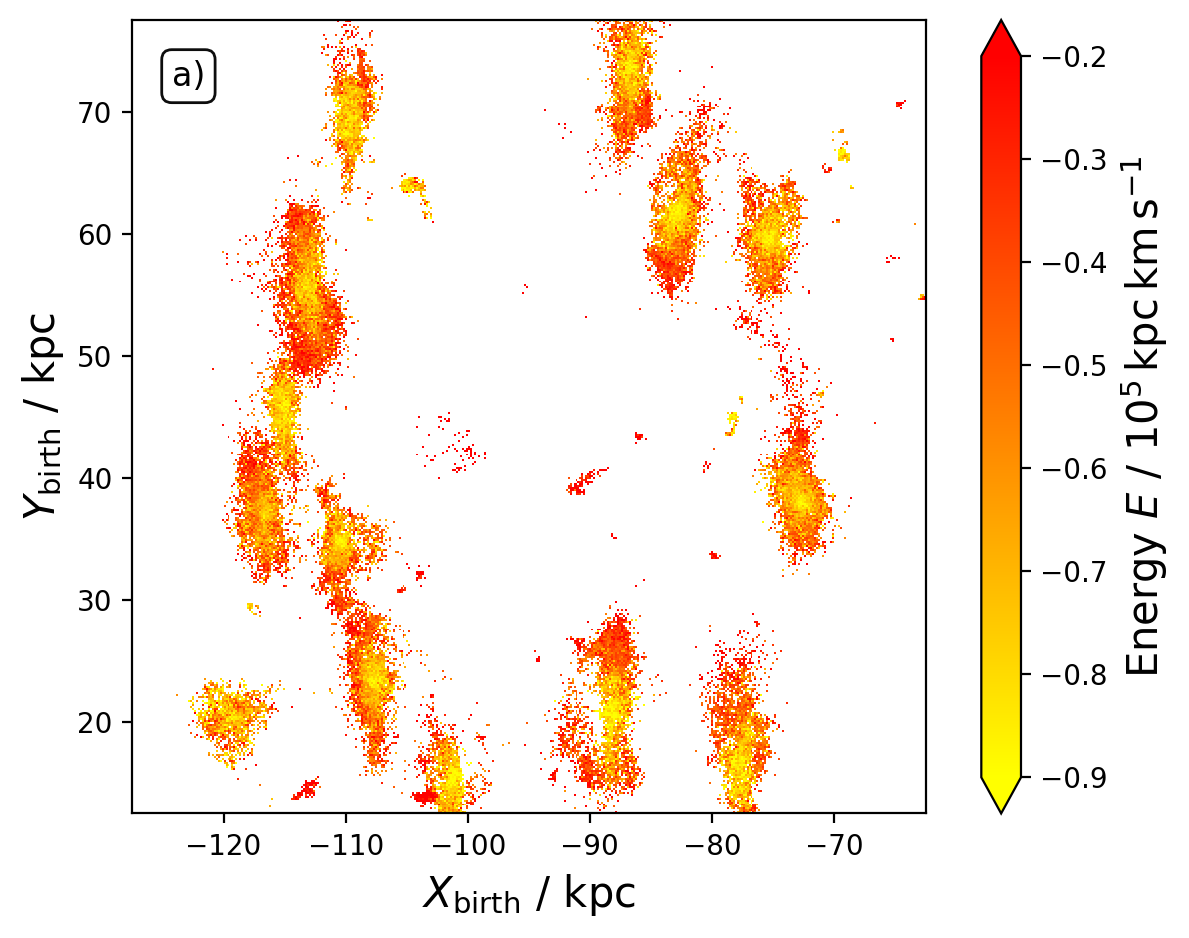
\includegraphics[width=\columnwidth]{figures/fellowship.png}
    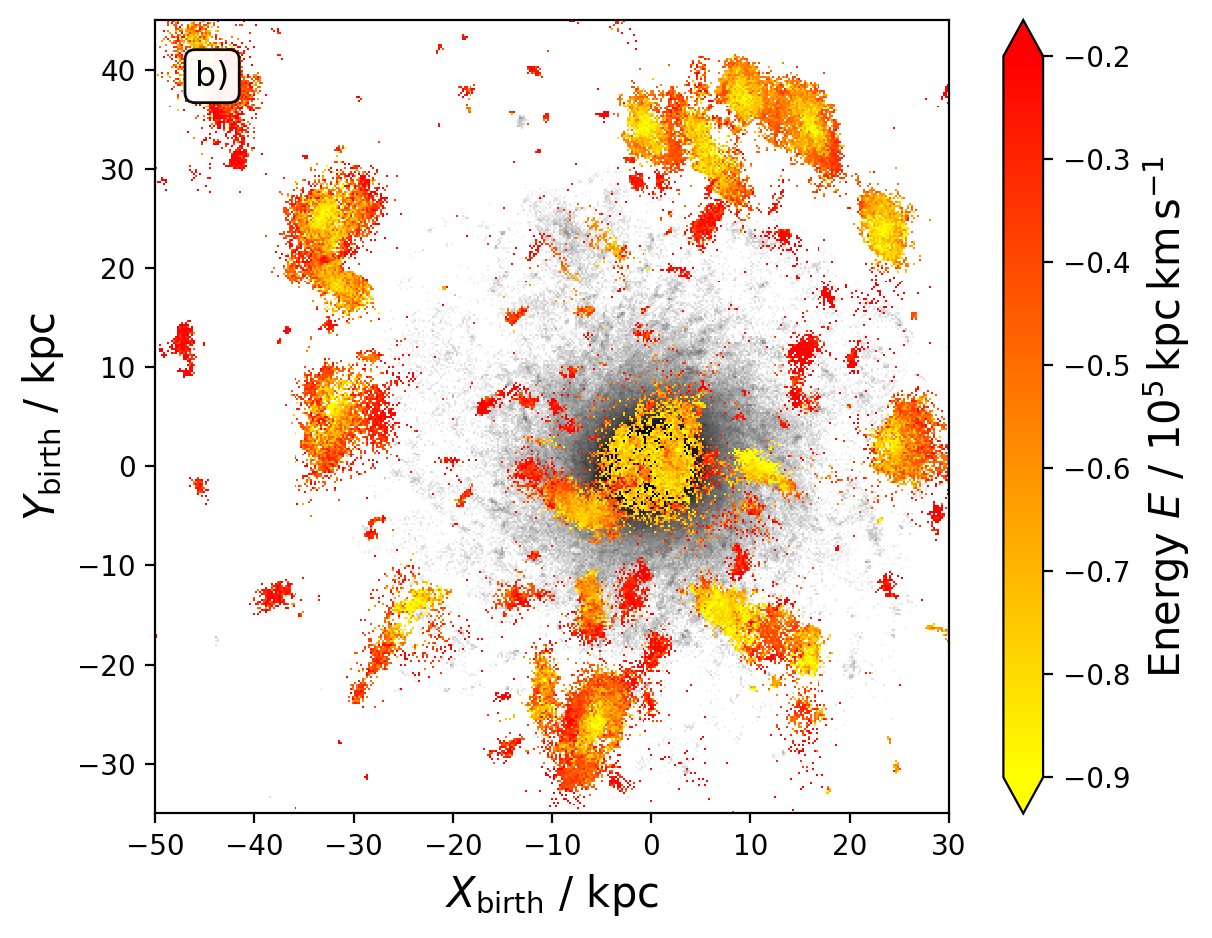
\includegraphics[width=\columnwidth]{figures/mount_doom.png}
    \caption{Birth positions (determined in batches of $100\,\mathrm{Myr}$) coloured by present-day orbit energy, both before the major merger (top) and just before and during the merger (bottom), with the main galaxy's birth positions visible in greyscale \href{https://github.com/svenbuder/gse_nihaouhd/tree/main/figures}{\faGithub}.}
    \label{fig:fellowship_and_mount_doom}
\end{figure}

A major motivation of our study is to investigate if there is any memory of the birth positions of accreted stars left in their orbits. \citet{Skuladottir2025} approached this question forward-looking, by tagging the radius of particles within the smaller galaxy in the simulation by \citet{Mori2024} before the merger and then tracing the time of pericenter passages and present-day orbit properties. In a variation of this approach, our post-processing of birth positions allows us to simply use the birth positions and colour them by their present-day orbit energies. By focussing on two specific regions of birth positions in the $X_\mathrm{birth}$ vs. $Y_\mathrm{birth}$ direction in Fig.~\ref{fig:fellowship_and_mount_doom}, we are effectively tracing the star formation (with a resolution of $\sim 100\,\mathrm{Myr}$) of the galaxy long before the merger (Fig.~\ref{fig:fellowship_and_mount_doom}a), as well as shortly before and during the merger (Fig.~\ref{fig:fellowship_and_mount_doom}b) with the main galaxy (grey background).

A striking feature of basically all de-facto snapshots of star formation is that the stars born in the outskirts now have high orbit energies (are coloured red), while the stars in the centres of each $100\,\mathrm{Myr}$ snapshot have low orbit energies (yellow). This is fully consistent with the conclusion drawn by \citet{Skuladottir2025} that stars born in the outskirts of the accreted galaxy have higher orbit energies and stars born in its core have lower orbit energies.

%%%%%%%%%%%%%%%%%%%%%%%%%%%%%%%%%%%%%%%%%%%%%%%%%
%%%%%%%%%%%%%%%%%%%%%%%%%%%%%%%%%%%%%%%%%%%%%%%%%
\section{Discussion}
\label{sec:discussion}

In this paper (Paper~I), we posed three key questions regarding the information recoverable from integrals-of-motion space. We now address these in turn. In Section~\ref{sec:discussion_finding_accreted_stars}, we discuss the efficiency and biases in selecting accreted stars. In Section~\ref{sec:discussion_strategy_finding_gse_members}, we consider the implications of these findings for future observational strategies to identify informative members of the Milky Way’s last major merger, \textit{GSE}. In Section~\ref{sec:discussion_memory}, we discuss what chemical and birth position memory of the progenitor galaxy is retained in integrals-of-motion space. Together, these results highlight both the opportunities and the limitations in reconstructing the Milky Way’s merger history from present-day phase-space substructures.

%%%%%%%%%%%%%%%%%%%%%%%%%%%%%%%%%%%%%%%%%%%%%%%%%
\subsection{Selection effects of accreted stars in integrals of motion space} \label{sec:discussion_finding_accreted_stars}

Our investigations in Section~\ref{sec:analysis_dynamic_properties} showed that the true extent of accreted stars in the simulated Milky Way analogue extends far into the inner galaxy, which is dominated by in-situ stars. This dominance explains why current observational research on the extent of accreted stars has identified a rather sharp transition at specific orbit energies or radial actions between in-situ and accreted stars of the \textit{GSE} \citep{Helmi2018, Feuillet2021, Monty2024}.

However, our results show that significantly more accreted stars are present with energies and radial actions below the observationally suggested limits in $E$ \citep{Helmi2018, Monty2024} and $J_R$ \citep{Feuillet2020, Feuillet2021}. Importantly, we find $42\,\mathrm{\%}$% and $28\,\mathrm{\%}$% of the accreted stars in regions that are dominated by in-situ stars on these low-energy orbits. The dynamical overlap of in-situ and accreted structures is significant and spectroscopic, that is, chemical insights are needed to separate in-situ from accreted stars \citep[for example][]{Das2020, Horta2021, Buder2022}.

While several accreted stars and even structures have been found in the inner Galaxy thanks to infrared spectroscopy \citep[for example][]{Horta2021}, this regions remains mostly out-of-reach for high-precision optical spectroscopy and partially even astrometry \citep{Queiroz2023}.

The current dedicated spectroscopic searches for accreted stars, which are typically limited to either the nearby or extended Solar neighbourhood \citep[for example][]{Nissen2010, Buder2022} or far away from the Galactic disc \citep{Naidu2020} can provide significant insights, but are expected to be not only incomplete but also significantly biased because of the subsample of \textit{GSE} stars that they are able to target. We remind ourselves that in the simulation, the spatial distribution of the lowest-energy accreted stars is limited to within $R_\mathrm{2D} = $$3.6_{-1.7}^{+1.7}\,\mathrm{kpc}$% and $Z = $$0.0_{-1.3}^{+1.3}\,\mathrm{kpc}$% (see Figs.~\ref{fig:xy_distribution_ezones} and \ref{fig:xz_distribution_ezones}). Assuming the distribution of accreted stars would be the same for the Milky Way, we would thus not expect a lot (or any) of the accreted stars with lowest energies to be present in the sample of 33 accreted stars in the Solar neighbourhood by \citet{Nissen2010}, but mainly those with $E > -0.57\times10^5\,\mathrm{kpc\,km\,s^{-1}}$, consistent with the sample studied by \citet{Skuladottir2025}. The same holds true for Milky Way halo studies \citep{Naidu2020}, which have helped us to better understand the substructure of accretion, but are expected to mostly target \textit{GSE} stars with $E > -0.77\times10^{5}\,\mathrm{kpc\,km\,s^{-1}}$.

Our simulation data suggests that we will find a currently under-represented subset of stars in the inner Galaxy, more specifically within its bulge region. Over the decades \citep[see for example][for a review]{Barbuy2018}, this dense region has been the target of several dedicated spectroscopic studies \citep[for example][]{Ness2013, Bensby2017, Lucey2019}. This raises the question if some accreted stars have already been observed by chance. \citet{Ness2013, Ness2013b}, for example, have identified specific overdensities in the metallicity distribution functions of the bulge region (i.e., below the center at $b = -5\,\mathrm{deg}$), namely at $\mathrm{[Fe/H]} \in [-1.73, -1.16, -0.66, -0.26, +0.12]$ with typical spreads of $\pm0.11-0.15$ \citep[see also][]{Portail2017}. Despite some differences between the actual peak positions \citep[compare for example Fig.~4 by][]{Barbuy2018}, different studies agreed with the presence of multiple overdensities. \citet{Bensby2017} found the second-lowest metallicity peak around $\mathrm{[Fe/H]} = -1.09$. \citet{Portail2017} also found a peak at $-1.18\pm 0.14$ with less (to no) net rotation, reminiscent of the characteristic [Fe/H] and $L_Z$ distribution of accreted stars. 

When focusing on the inner region of the Milky Way analogue ($R_\mathrm{2D} < 3.6\,\mathrm{kpc}$ and $\vert Z\vert < 1.3\,\mathrm{kpc}$), we also find a multi-modal metallicity distribution (see Fig.~\ref{fig:fe_h_histogram_inner_galaxy}a). The distribution is overall shifted to higher [Fe/H] values than the Milky Way by $\sim+0.3\,\mathrm{dex}$ compared to the measurements in the Milky Way bulge (see above). Taking this into account, we would expect the accreted stars to contribute mainly to the peak around $\sim-0.8$. We can confirm this when selecting the accreted stars of the simulation (golden in Fig.~\ref{fig:fe_h_histogram_inner_galaxy}a and zoomed in vertically for better visibility in Fig.~\ref{fig:fe_h_histogram_inner_galaxy}b). What strikes us here is the limited contribution of accreted stars to the inner galaxy (only $2\,\mathrm{\%}$%) but especially to the peak itself. This suggests two things: firstly that the amount of accreted stars distributed in the inner galaxy is insignificant (on a relative level) and secondly that there are still stars formed with the same, outstanding iron abundance as the accreted stars. A simple explanation could be that these particular stars formed from gas of the accreted galaxy -- an exciting avenue for quantifying the amount of metal-poor gas brought in by the accreted galaxy \citep{Buck2023}. This hypothesis should be followed up in a future study that dives into the detailed tracing of the gas of the simulation during the merger. In any case, we do note that the number of stars born with this iron abundance -- and in particular those contributing to the bump around $\mathrm{[Fe/H] \sim -0.75}$ in the simulation -- appears insignificant compared to the rest of stars in this inner region. A blind survey of 100 stars in this region would be expected to only find 2 accreted stars on average, whereas throughout the whole Galaxy, one would expect to find 9 (compare the contributions of accreted stars to the overall metallicity distribution function in Figs.~\ref{fig:fe_h_histogram_inner_galaxy}a and \ref{fig:fe_h_histogram_inner_galaxy}c).

\begin{figure}
    \centering
    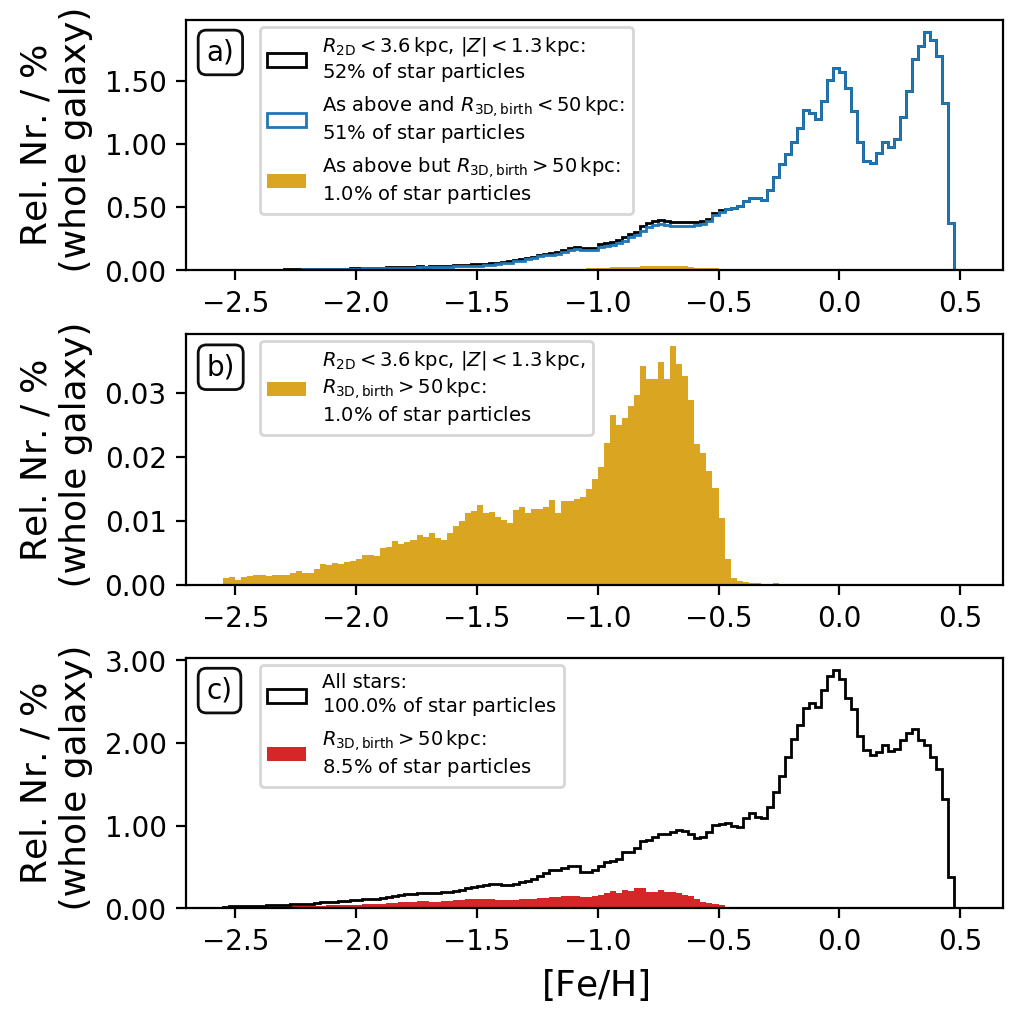
\includegraphics[width=\columnwidth]{figures/fe_h_histogram_inner_galaxy.png}
    \caption{Metallicity distribution functions (relative to total number of stars in the galaxy). Top panel shows the distribution of the inner $R_\mathrm{3D} < 3.6\,\mathrm{kpc}$ and how in-situ (blue) and accreted populations (golden) contribute to it. Panel b) is showing the same golden distribution of accreted stars as panel a), but zooming in to see more details. Panel c) shows the distribution of the whole galaxy (black) and all accreted stars (red) \href{https://github.com/svenbuder/gse_nihaouhd/tree/main/figures}{\faGithub}.}
    \label{fig:fe_h_histogram_inner_galaxy}
\end{figure}

The question therefore arises, if we perhaps have not actually found the core of the \textit{GSE} progenitors yet, since they are so well hidden in the centre of our Galaxy. While focussing on a larger metallicity-range in the metal-poor inner bulge, we note that \citet{Lucey2022} only found a small number and percentage of stars with accretion-like, sub-solar [Al/Fe] and [Mn/Fe] in their sample (see their Figs.~7 and 8). These stars certainly should be followed up to identify if they are part of the accreted population of the \textit{GSE} \citep[see also][]{Kunder2025}.

An observation that has previously been debated as a potential finding of the core of the last major merger of the Milky Way was the Heracles substructure \citep{Horta2021}, with some of the lowest energies of accreted stars found so far. While some researchers have argued that its seemingly distinct separation from the \textit{GSE} in the $L_Z$ vs. $E$ could have been caused by bar interactions \citep{Dillamore2025}, our findings from the simulation suggest that its metallicity (relative to the \textit{GSE}) is in fact too low to be part of the same system. We thus agree with \citet{Horta2021} that this system is likely a separate accretion event within the Milky Way.

Looking into the near future, the 4MOST survey's 4MIDABLE consortium surveys of the inner galaxy \citep{4MOST_HR_DiskBulge, 4MOST_LR_DiskBulge} will observe millions of stars towards this region. If the last major merger in our Milky Way is comparable to the one in our analogue simulation, we expect these surveys to observe a considerable number of accreted stars. If one could preselect stars with $\mathrm{[Fe/H]} < -0.5$ for spectroscopic follow-up to measure Na or Al as well as Mg and Mn, our simulation data suggests an increase of the ratio of accreted stars in the inner Galaxy from $2\,\mathrm{\%}$% to $10\,\mathrm{\%}$%. The efficiency of such preselections, for example via photometric observations \citep[for example from the Pristine and SkyMapper surveys][]{Starkenburg2017, DaCosta2019} or spectrophotometric observations \citep[for example by combining \textit{Gaia} BP/RP spectrophotometry and narrow-band Pristine photometry][]{Martin2024} have already been shown in the inner galaxy \citep[for example by][with the Pristine Inner Galaxy Survey]{Arentsen2020, Arentsen2020b} and could also be implemented for future observations, for example of the APOGEE survey in the infrared towards the inner galaxy \citep{Santana2021}.

Subsequently we discuss why such observations could be key for our understanding of the last major merger of the Milky Way by allowing us to better quantify the amount of low-energy \textit{GSE} members.

%%%%%%%%%%%%%%%%%%%%%%%%%%%%%%%%%%%%%%%%%%%%%%%%%
\subsection{The importance of finding low-energy \textit{GSE} members} \label{sec:discussion_strategy_finding_gse_members}

What could be the potential impact of missing out on the hidden low-energy members of the \textit{GSE}? The detailed impact of the major merger will lie in the impact of the accreted gas and stars onto the chemical make-up and rotation of the Galaxy as well as the merger configuration and pathway. Two general galaxy properties -- galaxy mass or mean metallicity -- are often used to quantify a galaxy and its potential impact during a merger. With the observationally found mass-metallicity relation \citep[for example][]{Gallazzi2005, Kirby2013}, these numbers are correlated and allow to roughly estimate the mass of a system from its metallicity and vice versa. In the Milky Way, this relation has been confirmed with surviving smaller galaxies \citep{Kirby2013} and then used to estimate the masses of disrupted galaxies by comparison \citep[for example][]{Helmi2018} -- in addition to dynamical mass estimates from simulations that recovered the dynamical signatures of the disrupted galaxies \citep[for example][]{Naidu2022b}.

By comparing the mass-metallicity relations of observed surviving and (partially or fully) disrupted dwarf galaxies, \citet{Naidu2022b} uncovered a significant offset between them, with the latter's metallicities being on average 0.30 lower, thus questioning the universality of the mass-metallicity relation. If the selection efficiency described in the prior section is indeed biased, this raises the question, if this bias is possibly, at least partially, introduced by selection biases. Beyond the biases for \textit{GSE} \citep{Skuladottir2025}, we are wondering if the [Fe/H] estimates of surviving dwarf galaxies could be biased by the analysis of stars in their cores (and less so their outskirts), whereas the [Fe/H] estimates of disrupted dwarf galaxies could be biased towards lower values by the stars in their previous outskirts, rather than their more metal-rich cores (which our simulations suggest to be more likely embedded in the inner galaxy regions dominated by in-situ stars). To visualise this point, we are recreating the mass-metallicity relation as shown by \citet{Naidu2022b} in Fig.~\ref{fig:mzr_different_selections}. To this figure, we add the median [Fe/H] values for the four different energy zones of the accreted stars in our simulation (with yellow to dark red corresponding to the lowest to highest energy zones from Fig.~\ref{fig:fe_h_histograms}). We indeed see that when selecting preferentially (or even only) the the higher energy samples, we tend to infer a lower [Fe/H]. The lower-energy samples would increase the average median [Fe/H]. We also notice that shape -- in particular the non-Gaussianity -- of the metallicity distribution functions of a galaxy needs to be included into this figure for both surviving and disrupted dwarf galaxies, rather than the currently used mean or median [Fe/H].

In a future project, we will perform a detailed re-assessment of the mass-metallicity relation under full consideration of the metallicity distributions and inclusion of potential biases.

\begin{figure}
    \centering
    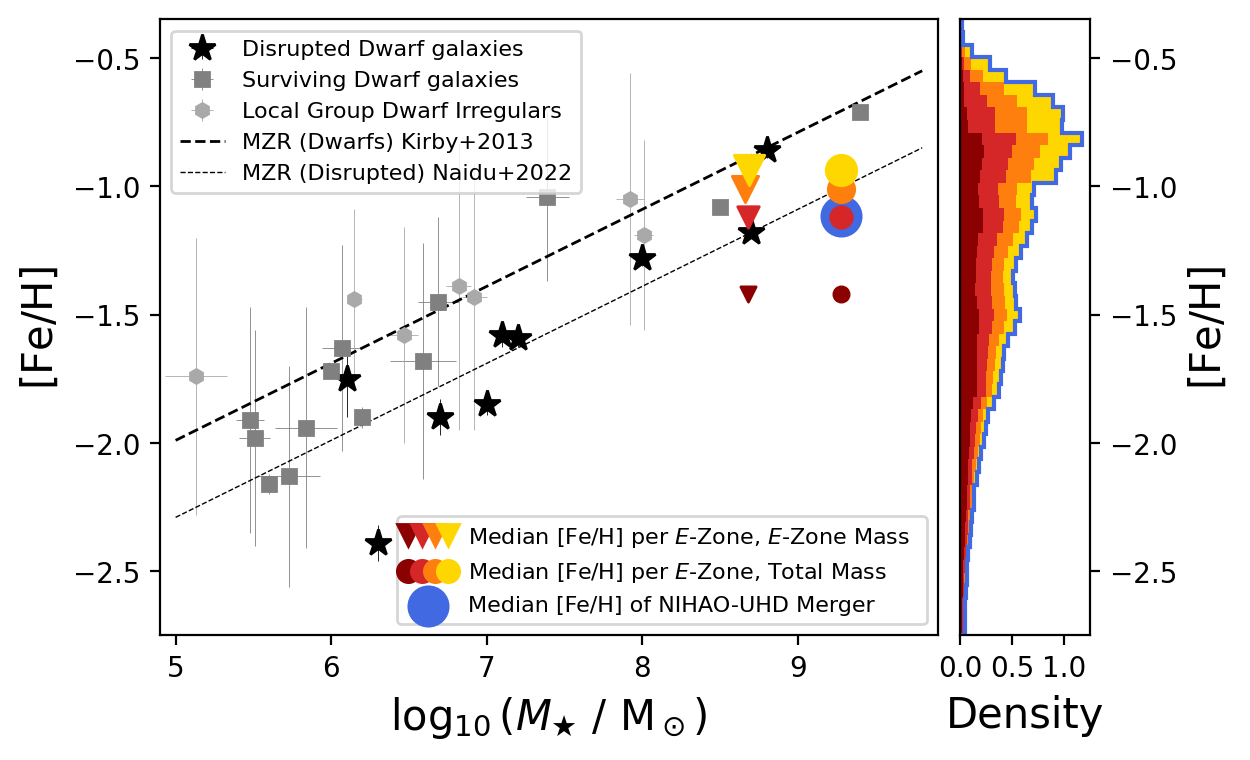
\includegraphics[width=\columnwidth]{figures/mzr_different_selections.png}
    \caption{Mass-metallicity relations (dashed lines) for different galaxies and selections. We list both reported measurements of disrupted (black star symbols), surviving  (grey squares), and irregular dwarf galaxies (grey circles) by \citet{Kirby2013} and \citet{Naidu2022b}. For the major merger of the NIHAO-UHD Milky Way analogue we show both the median [Fe/H] and total mass for the whole merger (blue dot), and median [Fe/H] of the different energy zones vs. the total merger mass (coloured dots); and only the masses of star particles in the individual energy zones (coloured triangles). Right panel shows the stacked histograms of the different metallicity distributions following the same colour code \href{https://github.com/svenbuder/gse_nihaouhd/tree/main/figures}{\faGithub}.}
    \label{fig:mzr_different_selections}
\end{figure}

%%%%%%%%%%%%%%%%%%%%%%%%%%%%%%%%%%%%%%%%%%%%%%%%%
\subsection{Chemical and birth position memory of the progenitor galaxy in integrals of motion space} \label{sec:discussion_memory}

Throughout our analysis in Section~\ref{sec:analysis_chemodynamic_memory}, we have investigated if we can find the same patterns from the observational study by \citet{Skuladottir2025} that accreted stars with different orbit energies carry both chemical and birth position memory.

Indeed, we have found correlations of present-day orbit energy and metallicity (Fig.~\ref{fig:fe_h_histograms}) as well as chemical enhancement of several individual elements (Fig.~\ref{fig:xfe_feh_zones}), but also a correlation with present-day orbits (Figs.~\ref{fig:xy_distribution_ezones} and \ref{fig:xz_distribution_ezones}) and most importantly birth positions (Fig.~\ref{fig:fellowship_and_mount_doom}). While these findings are all in agreement with the findings by \citet{Skuladottir2025} at face value, here we want to discuss a few more subtle differences that we note because of our larger sample size that also reaches towards the lower-energy regions and thus the core of the major merger galaxy.

Because of the low number of only 33 targets, \citet{Skuladottir2025} could only subdivide their sample into two groups. To quantify the abundance differences between the groups beyond computing abundance offsets, they fitted linear functions in [Fe/H] vs. [X/Fe] space and were able to identify both overall offsets and linear, that is, metallicity-dependent trends. However, the abundance trends of our simulation in Fig.~\ref{fig:xfe_feh_zones} show non-linear trends, which would be insufficiently covered by linear functions. In particular, we note a shift of the skewed metallicity distribution function with decreasing orbit energy from metal-poor to metal-rich. \citet{Skuladottir2025} have in fact made a similar discovery in their research, when assessing the impact of the energy cut onto the metallicity distribution function (see their Appendix~A), where moving their energy cut to lower energies limits the sample to quite high $\mathrm{[Fe/H]} \gtrsim -0.9$ and reveals two significantly different distributions, in line with our findings. Again in line with our findings, they found significantly different abundance patterns, especially for $\mathrm{[Fe/H]} > -1$.

Because of the changing metallicity distribution function and some non-linear trends in [X/Fe] in our larger -- but simulated -- sample, we believe that future investigation of observed abundance trends -- in the best case with larger samples across a diverse energy range -- should aim to go beyond the fitting of linear trends to these distributions as done by \citet{Skuladottir2025}.

Our investigations confirm the conclusions drawn by \citet{Skuladottir2025}, that the lower-energy stars were born in the inner parts of the now-accreted galaxy, whereas higher-energy stars were born in its outskirts. Similarly, the combination of our investigation and the findings by \citet{Skuladottir2025} suggests that the \text{GSE} was a galaxy with a noticeable radial metallicity gradient (for a visual impression look at the smaller galaxy in Fig.~\ref{fig:trace_star_formation_xy_feh} around $9.5-10.0\,\mathrm{Gyr}$). Our investigation of a cosmological zoom-in simulation thus supports the finding by \citet{Skuladottir2025} that the \text{GSE} progenitor had a clear radial metallicity gradient. This provides rare direct evidence of internal chemical structure in an accreted galaxy and is yet another confirmation that \text{GSE} likely experienced extended, inside-out star formation before merging with the Milky Way.

%%%%%%%%%%%%%%%%%%%%%%%%%%%%%%%%%%%%%%%%%%%%%%%%%
%%%%%%%%%%%%%%%%%%%%%%%%%%%%%%%%%%%%%%%%%%%%%%%%%
\section{Conclusions}
\label{sec:conclusions}

We have used a high-resolution NIHAO-UHD cosmological simulation to study the last major merger of a Milky Way analogue, addressing three key questions:

First (Sec.~\ref{sec:discussion_finding_accreted_stars}), the present-day orbital properties of accreted stars correlate with their birth radii within the progenitor galaxy.

Second (Secs.~\ref{sec:discussion_memory} and \ref{sec:discussion_strategy_finding_gse_members}), these correlations arise from abundance gradients within the progenitor. Lower-energy stars, now more strongly bound to the Milky Way, formed in the core of the accreted galaxy and are systematically more metal-rich and chemically enhanced. This supports the scenario of \citet{Skuladottir2025} and demonstrates that chemodynamical memory is preserved across the merger. However, accreted stars also extend to much lower orbital energies and radial actions than previously inferred. As a consequence, selection methods in integrals-of-motion space \citep{Helmi2018, Feuillet2021, Monty2024} systematically miss stars from the progenitor’s core. Progenitor reconstructions are therefore biased toward the chemically metal-poor outskirts. These biases may even help explain differences in the mass–metallicity relation between surviving and disrupted dwarf galaxies \citep{Naidu2022}, offering a testable prediction for future work.

Third, our analysis shows that current selection functions alone are insufficient to capture the full abundance distribution of the progenitor. Future survey strategies must target inner-Galaxy stars to recover the missing, chemically enriched core population.

Our findings highlight the power of cosmological simulations to quantify biases introduced by observational selection functions, and to guide strategies for building a more representative census of accreted stars in the Milky Way.

% \clearpage
%%%%%%%%%%%%%%%%%%%%%%%%%%%%%%%%%%%%%%%%%%%%%%%%%
%%%%%%%%%%%%%%%%%%%%%%%%%%%%%%%%%%%%%%%%%%%%%%%%%
\section*{Acknowledgments}

We acknowledge the traditional owners of the land on which the ANU stands, the Ngunnawal and Ngambri people. We pay our respects to elders past, and present and are proud to continue their tradition of surveying the night sky and its mysteries to better understand our Universe. SB acknowledges support from the Australian Research Council under grant number DE240100150.
TB's contribution to this project was made possible by funding from the Carl Zeiss Stiftung. \'{A}S~acknowledges funding from the European Research Council (ERC) under the European Union’s Horizon 2020 research and innovation programme (grant agreement No. 101117455).

%%%%%%%%%%%%%%%%%%%%%%%%%%%%%%%%%%%%%%%%%%%%%%%%%
%%%%%%%%%%%%%%%%%%%%%%%%%%%%%%%%%%%%%%%%%%%%%%%%%
\section*{Data Availability}

All code to reproduce the analysis and figures can be publicly accessed via \url{https://github.com/svenbuder/gse_nihaouhd}.

The used simulation snapshot can be publicly accessed as FITS file via \url{https://github.com/svenbuder/preparing_NIHAO}. Original data, more snapshots and other galaxies can be found at \url{https://tobias-buck.de/#sim_data}. We encourage interested readers to get in contact with the authors for full data access and advice for use and cite \citet{Buck2020b, Buck2021}.

\section*{Software}

The research for this publication was coded in \textsc{python} (version 3.12.11) and included its packages
\textsc{astropy} \citep[v. 7.1.0;][]{Robitaille2013,PriceWhelan2018},
\textsc{hyppo} \citep[v. 0.5.2;][]{hyppo},
\textsc{IPython} \citep[v. 9.1.0;][]{ipython},
\textsc{matplotlib} \citep[v. 3.10.3;][]{matplotlib},
\textsc{NumPy} \citep[v. 2.2.6;][]{numpy}, as well as
\textsc{scipy} \citep[v. 1.16.0;][]{Scipy}.
We further made use of \textsc{topcat} \citep[version 4.7;][]{Taylor2005};
 
%%%%%%%%%%%%%%%%%%%%%%%%%%%%%%%%%%%%%%%%%%%%%%%%%
%%%%%%%%%%%%%%%%%%%%%%%%%%%%%%%%%%%%%%%%%%%%%%%%%
\bibliographystyle{mnras}
\bibliography{bib}

%%%%%%%%%%%%%%%%%%%%%%%%%%%%%%%%%%%%%%%%%%%%%%%%%
%%%%%%%%%%%%%%%%%%%%%%%%%%%%%%%%%%%%%%%%%%%%%%%%%
% \clearpage
\appendix

\section{Additional Information}

\begin{figure}
    \centering
    % \includegraphics[width=0.49\linewidth]{figures/fraction_accreted_in_situ_lz.png}
    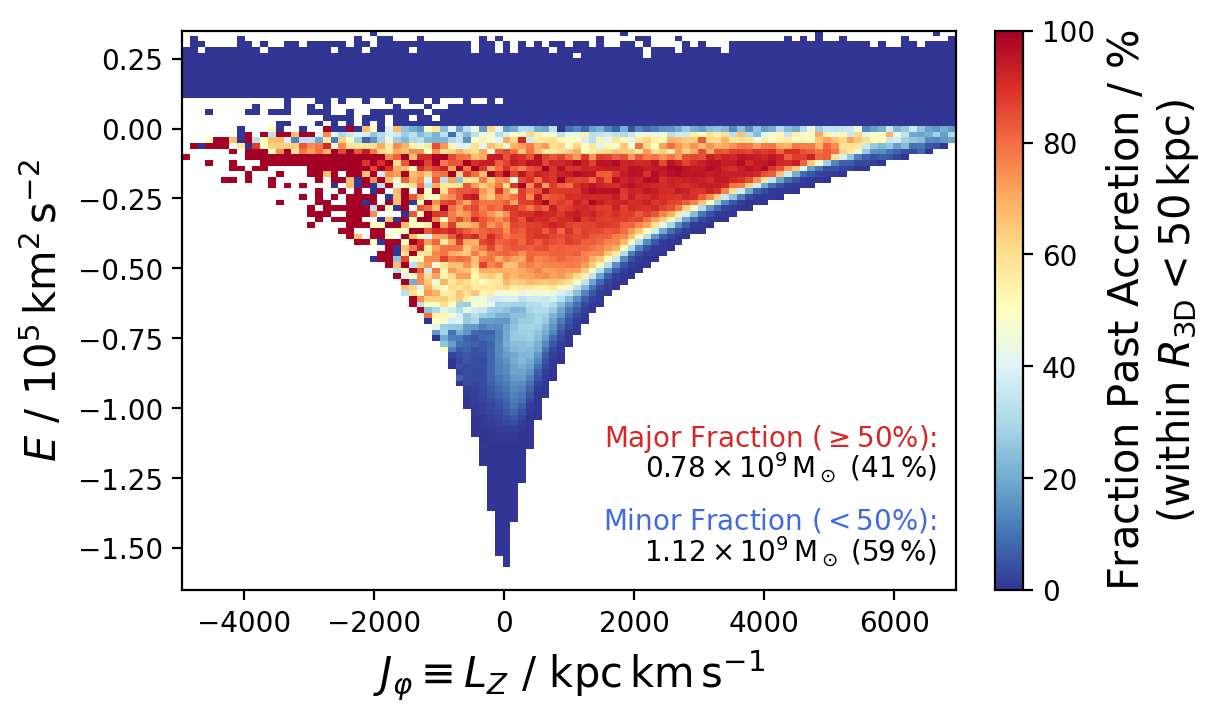
\includegraphics[width=\columnwidth]{figures/fraction_accreted_in_situ_lz_e_total.png}
    % 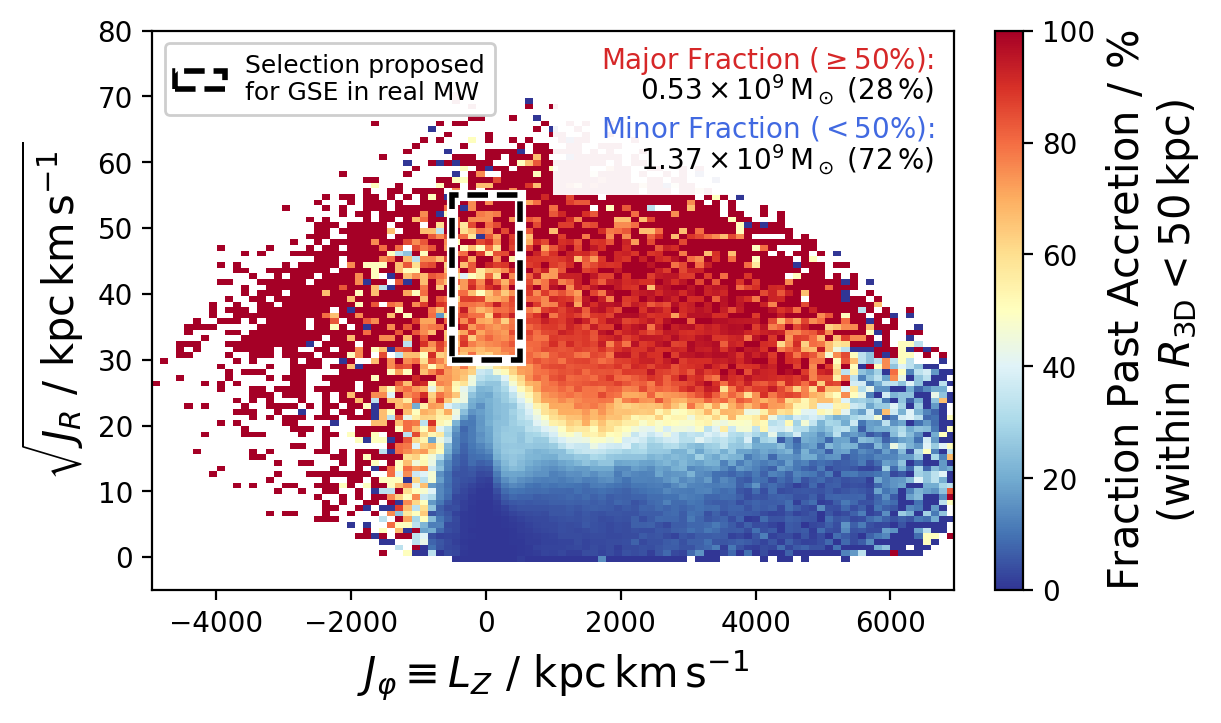
\includegraphics[width=0.49\linewidth]{figures/fraction_accreted_in_situ_lz_jr.png}
    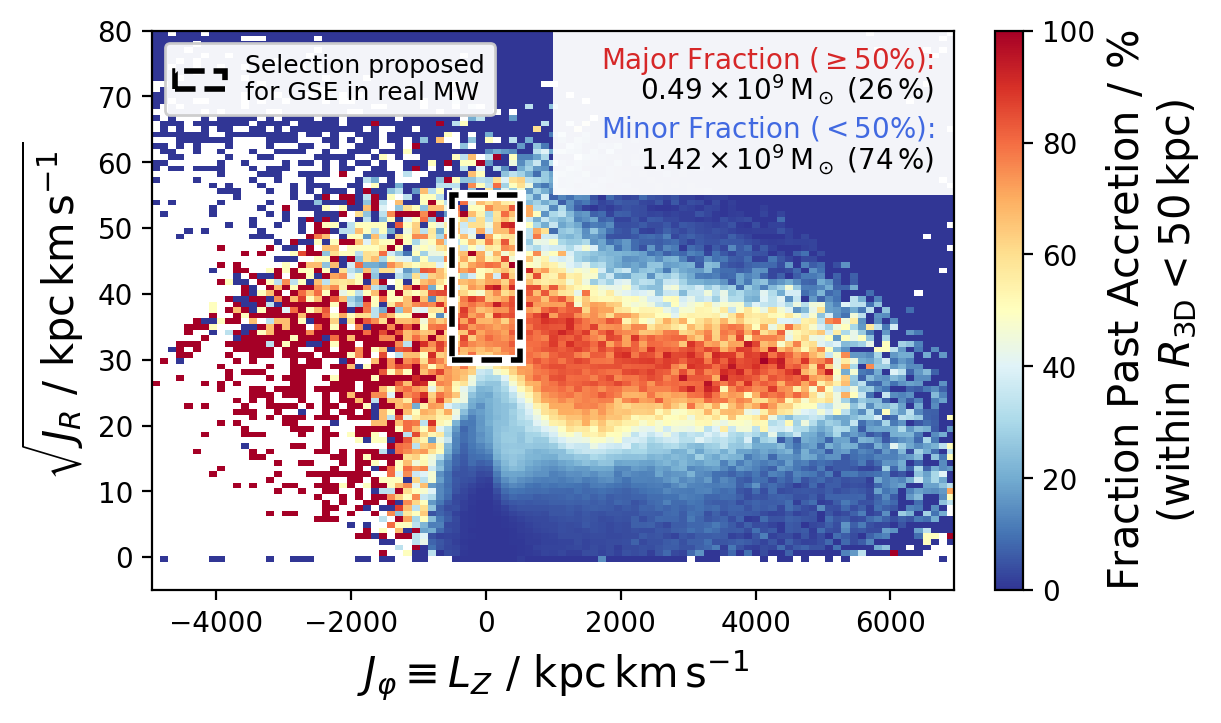
\includegraphics[width=\columnwidth]{figures/fraction_accreted_in_situ_lz_jr_total.png}
    \caption{A version of Fig.~\ref{fig:fraction_accreted_in_situ_lz}, but calculating fractions with respect to all star particles.}
    \label{fig:fraction_accreted_in_situ_lz_total}
\end{figure}

\begin{table*}
    \centering
    \caption{Spatial and age selection used to identify individual (and clean) overdensities in birth positions for Fig.~\ref{fig:tracing_xyz_birth_3}.}
    \begin{tabular}{cccccccccc}
\hline \hline
Property & $X$ Range & $Y$ Range & $Z$ Range & Age Range & $X$ Center & $Y$ Center & $Z$ Center & Median Age & Median [Fe/H] \\
Unit & $\mathrm{kpc}$ & $\mathrm{kpc}$ & $\mathrm{kpc}$ & $\mathrm{Gyr}$ & $\mathrm{kpc}$ & $\mathrm{kpc}$ & $\mathrm{kpc}$ & $\mathrm{Gyr}$ & $\mathrm{dex}$ \\
\hline
1 & -40..-25 & 10..33 & -175..-155 & 11.0..13.0 & -32 & 20 & -166 & $12.24\pm0.03$ & $-1.50\pm0.18$ \\
2 & -19..-9 & 46..68 & -174..-160 & 10.9..12.9 & -13 & 56 & -166 & $11.92\pm0.03$ & $-1.27\pm0.12$ \\
3 & 0..12 & 20..45 & -176..-164 & 10.8..12.8 & 6 & 32 & -169 & $11.79\pm0.03$ & $-1.21\pm0.17$ \\
4 & -53..-38 & 30..60 & -166..-144 & 10.7..12.7 & -43 & 39 & -160 & $11.72\pm0.04$ & $-1.36\pm0.24$ \\
5 & -80..-65 & 32..52 & -154..-130 & 10.6..12.6 & -73 & 39 & -143 & $11.60\pm0.04$ & $-1.17\pm0.15$ \\
6 & -79..-72 & 50..66 & -142..-124 & 10.5..12.5 & -75 & 60 & -132 & $11.48\pm0.04$ & $-1.12\pm0.16$ \\
7 & -86..-79 & 50..75 & -132..-114 & 10.4..12.4 & -83 & 61 & -121 & $11.37\pm0.04$ & $-1.14\pm0.17$ \\
8 & -92..-80 & 65..90 & -115..-98 & 10.3..12.3 & -87 & 74 & -106 & $11.29\pm0.03$ & $-1.12\pm0.18$ \\
9 & -114..-106 & 64..81 & -86..-72 & 10.2..12.2 & -109 & 70 & -80 & $11.16\pm0.03$ & $-0.99\pm0.20$ \\
10 & -120..-107 & 45..64 & -86..-66 & 10.1..12.1 & -113 & 54 & -75 & $11.06\pm0.04$ & $-1.04\pm0.15$ \\
11 & -117..-112 & 39..51 & -71..-62 & 9.9..11.9 & -115 & 46 & -67 & $10.96\pm0.03$ & $-0.92\pm0.14$ \\
12 & -120..-100 & 29..46 & -62..-44 & 9.8..11.8 & -116 & 36 & -52 & $10.82\pm0.07$ & $-0.98\pm0.12$ \\
13 & -113..-103 & 14..30 & -61..-43 & 9.7..11.7 & -108 & 23 & -50 & $10.62\pm0.04$ & $-0.98\pm0.12$ \\
14 & -104..-98 & 8..25 & -50..-43 & 9.5..11.5 & -102 & 14 & -49 & $10.51\pm0.04$ & $-0.92\pm0.10$ \\
15 & -93..-84 & 12..32 & -66..-48 & 9.4..11.4 & -88 & 23 & -57 & $10.42\pm0.03$ & $-0.94\pm0.10$ \\
16 & -82..-73 & 11..29 & -63..-49 & 9.3..11.3 & -78 & 18 & -58 & $10.31\pm0.03$ & $-0.90\pm0.09$ \\
17 & -62..-53 & 9..34 & -69..-54 & 9.2..11.2 & -57 & 25 & -62 & $10.19\pm0.04$ & $-0.83\pm0.08$ \\
18 & -36..-20 & 17..33 & -73..-44 & 9.1..11.1 & -33 & 25 & -63 & $10.09\pm0.04$ & $-0.79\pm0.10$ \\
19 & -36..-20 & -10..15 & -73..-44 & 9.0..11.0 & -32 & 4 & -54 & $9.98\pm0.04$ & $-0.86\pm0.06$ \\
20 & -31..-19 & -25..-5 & -43..-28 & 8.9..10.9 & -24 & -14 & -36 & $9.88\pm0.04$ & $-0.74\pm0.09$ \\
21 & -12..0 & -35..-15 & -23..-6 & 8.8..10.8 & -6 & -26 & -15 & $9.75\pm0.02$ & $-0.81\pm0.07$ \\
22 & 9..19 & -34..-12 & 2..16 & 8.6..10.6 & 14 & -17 & 7 & $9.61\pm0.43$ & $-0.66\pm0.12$ \\
23 & 20..35 & -6..10 & 14..34 & 8.5..10.5 & 26 & 2 & 23 & $9.56\pm0.02$ & $-0.77\pm0.06$ \\
24 & 14..28 & 19..28 & 25..36 & 8.4..10.4 & 24 & 24 & 30 & $9.46\pm0.03$ & $-0.72\pm0.05$ \\
25 & 10..20 & 27..41 & 23..38 & 8.3..10.3 & 16 & 34 & 29 & $9.34\pm0.03$ & $-0.70\pm0.05$ \\
26 & 6..15 & 31..41 & 15..27 & 8.2..10.2 & 10 & 37 & 22 & $9.22\pm0.02$ & $-0.68\pm0.05$ \\
27 & -4..15 & 28..39 & 8..17 & 8.1..10.1 & -1 & 34 & 14 & $9.10\pm0.04$ & $-0.64\pm0.05$ \\
28 & -17..3 & 12..29 & -8..7 & 8.0..10.0 & -8 & 23 & -1 & $9.04\pm0.03$ & $-0.65\pm0.04$ \\
29 & -19..5 & -13..1 & -12..0 & 7.9..9.9 & -7 & -4 & -6 & $8.89\pm0.04$ & $-0.60\pm0.08$ \\
30 & -21..16 & -21..-10 & 3..10 & 7.8..9.8 & 8 & -15 & 8 & $8.80\pm0.03$ & $-0.57\pm0.06$ \\
31 & 3..27 & -6..3 & 2..11 & 7.7..9.7 & 11 & -1 & 5 & $8.70\pm0.03$ & $-0.50\pm0.03$ \\
32 & -23..19 & -16..13 & -4..5 & 7.6..9.6 & -5 & -2 & 0 & $8.62\pm0.36$ & $-0.49\pm0.07$ \\
\hline \hline
\end{tabular}

    \label{tab:birth_position_tabular}
\end{table*}

\begin{enumerate}[leftmargin=2em,labelwidth=0em]
    \item We provide both the initial selection and resulting average spatial and age ranges of the major accreted structure in Tab.~\ref{tab:birth_position_tabular}.
    \item Fig.~\ref{fig:fraction_accreted_in_situ_lz_total} shows the same distribution of stars in bins of $L_Z$ vs. $E$ and $L_Z$ vs. $\sqrt{J_R}$ as Fig.~\ref{fig:fraction_accreted_in_situ_lz}. In this version, we include ongoing accretion in addition to past accretion and in-situ formation when calculating the fractional contribution for each bin. 
    \item Fig.~\ref{fig:xz_distribution_ezones} shows the spatial distribution of accreted stars as Fig.~\ref{fig:xy_distribution_ezones}, but for the $X-Z$ direction.
      \item Fig.\ref{fig:additional_xfe_feh_zones} includes the chemical distribution of accreted stars beyond the ones already shown in Fig.~\ref{fig:xfe_feh_zones}. In addition to $\log(\mathrm{O/H}) + 12$ vs. $\log(\mathrm{N/O})$, they include the alpha-process elements O, Ne, Si, and S (behaving like the alpha-process element Mg), the odd-Z elements Na, Cl, and Cu (behaving like the odd-Z element Al), the iron-peak element Mn (behaving like the iron-peak element Ni), the neutron-capture elements Y, Ce, and Eu (behaving like the neutron-capture element Ba). For completeness, we also include C, Ti, and Zn. We neglect He, because it is modelled as a linear function of [Fe/H].
\end{enumerate}

\begin{figure*}
    \centering
    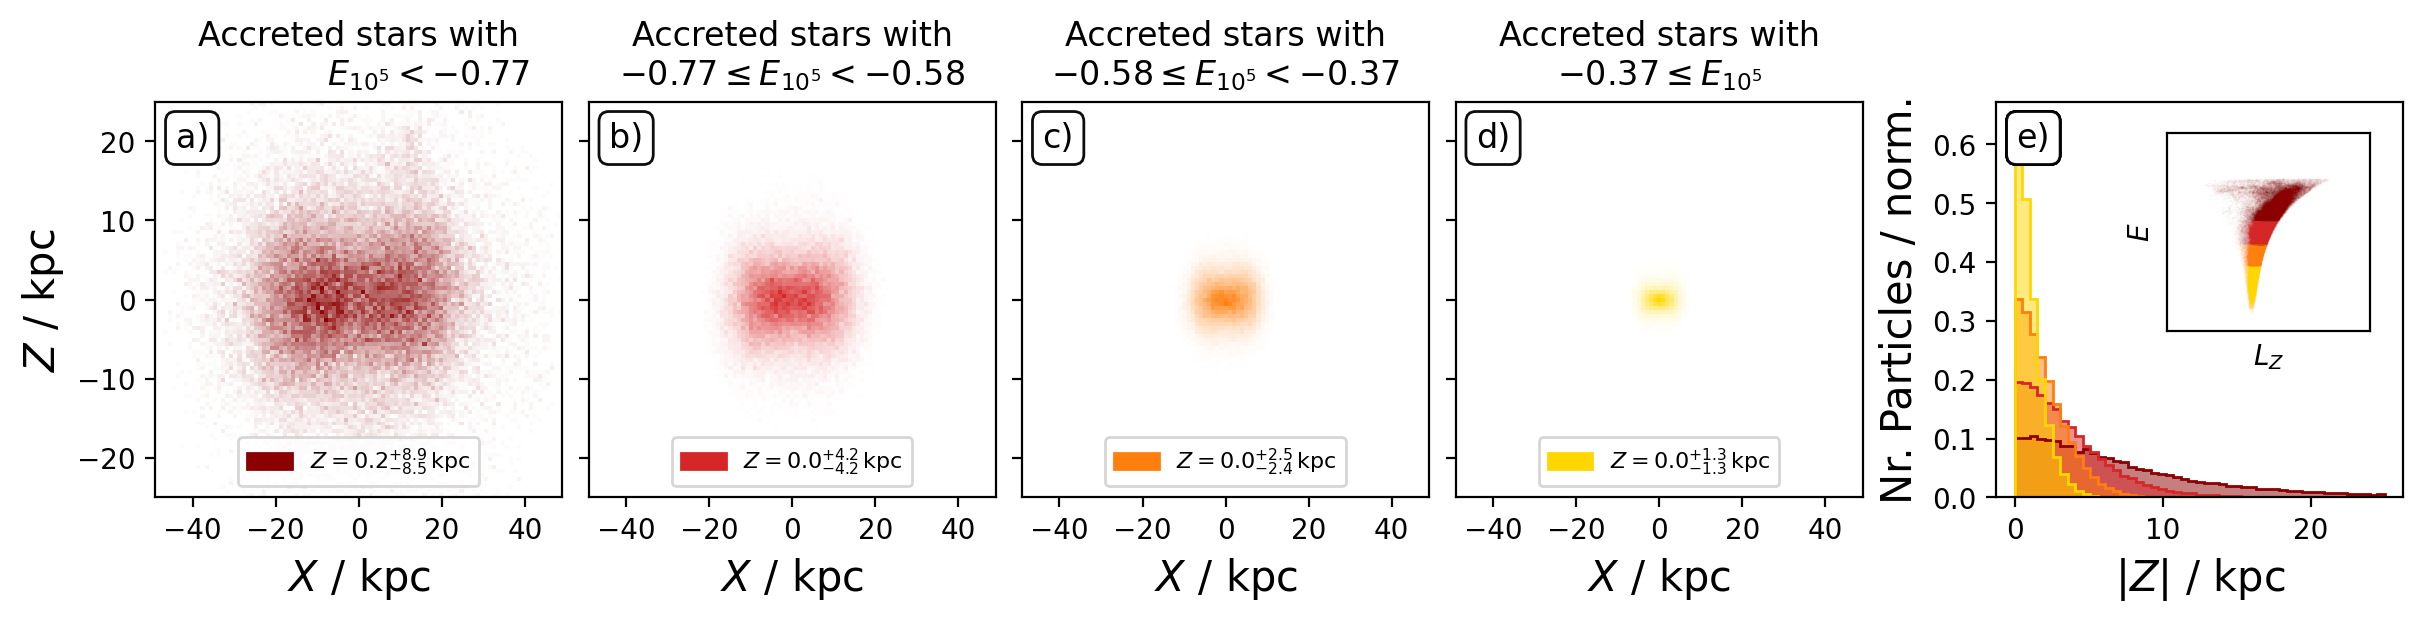
\includegraphics[width=\textwidth]{figures/xz_distribution_ezones.png}
    \caption{Present-day spatial distribution of accreted stars in the Galactocentric $X$-$Z$ plane. Panels a-d) show the density distribution of accreted stars with highest to lowest orbit energy quantiles. Panel legends list the 50th and 16th-84th percentiles of galactocentric height $Z$. Panel e) shows the absolute galactocentric height $\vert Z \vert$ distribution, and the inset visualises the $L_Z$ vs. $E$ selection \href{https://github.com/svenbuder/gse_nihaouhd/tree/main/figures}{\faGithub}.}
    \label{fig:xz_distribution_ezones}
\end{figure*}

\begin{figure*}
    \centering
    % 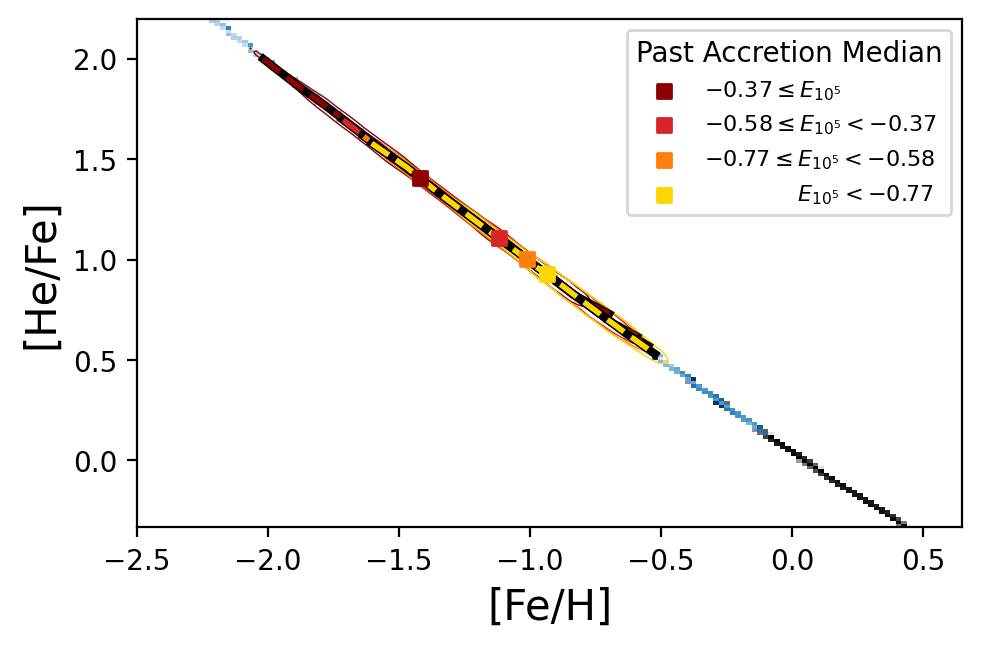
\includegraphics[width=0.33\textwidth]{figures/xfe_feh_zones_He.png}
    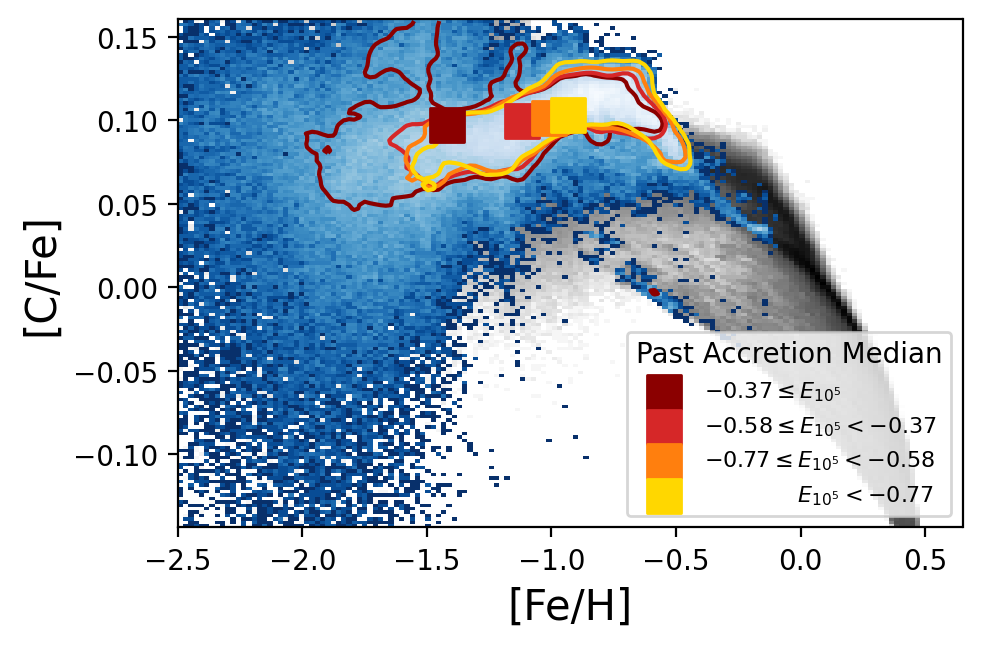
\includegraphics[width=0.33\textwidth]{figures/xfe_feh_zones_C.png}
    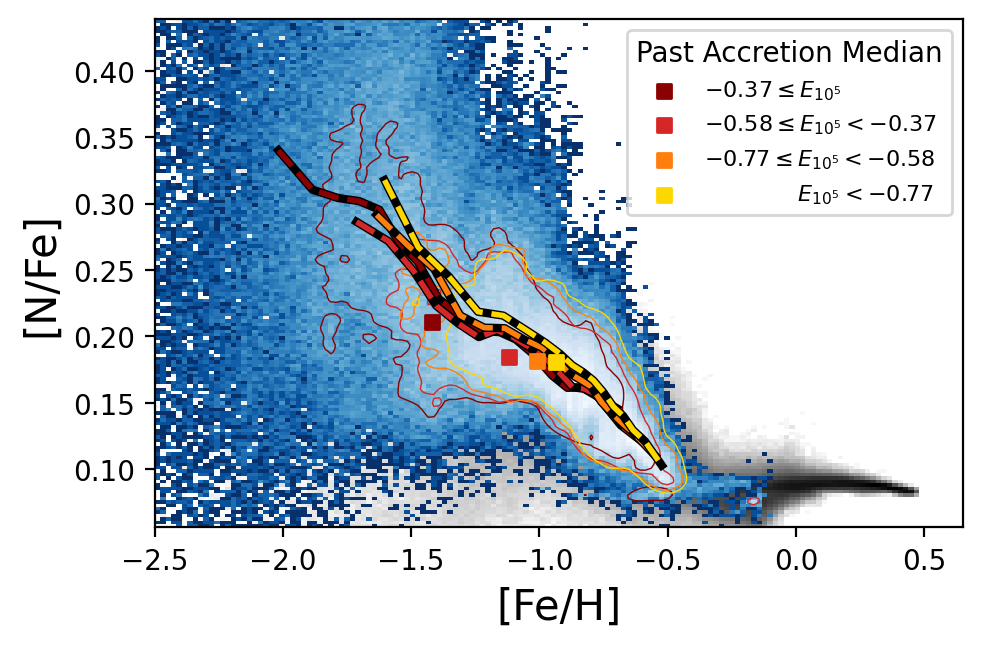
\includegraphics[width=0.33\textwidth]{figures/xfe_feh_zones_N.png}
    %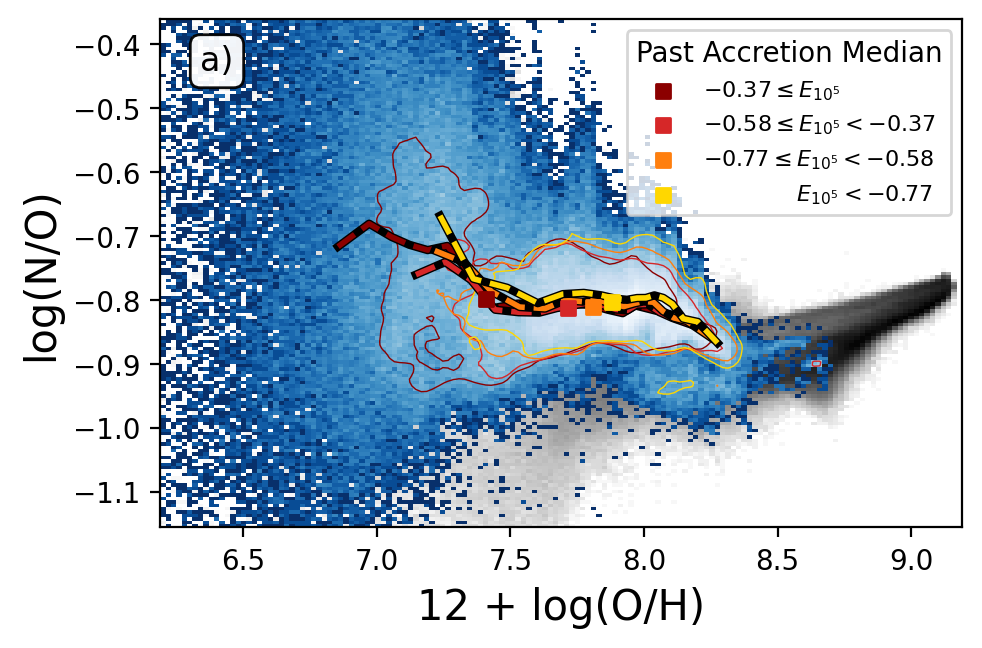
\includegraphics[width=0.33\textwidth]{figures/xfe_feh_zones_NO.png}
    % O == Mg
    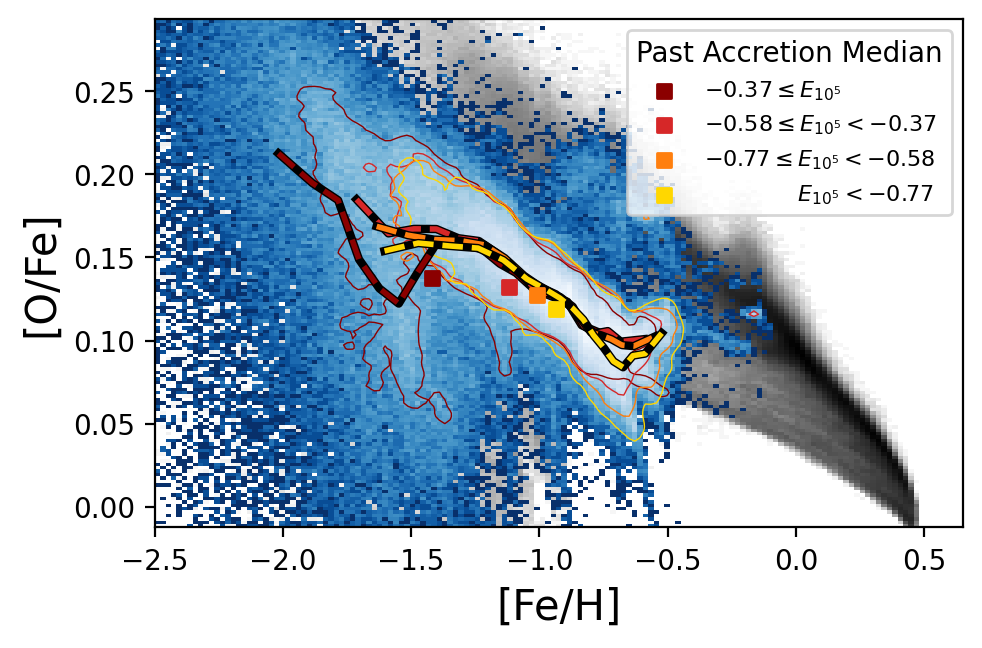
\includegraphics[width=0.33\textwidth]{figures/xfe_feh_zones_O.png}
    % Ne == Mg
    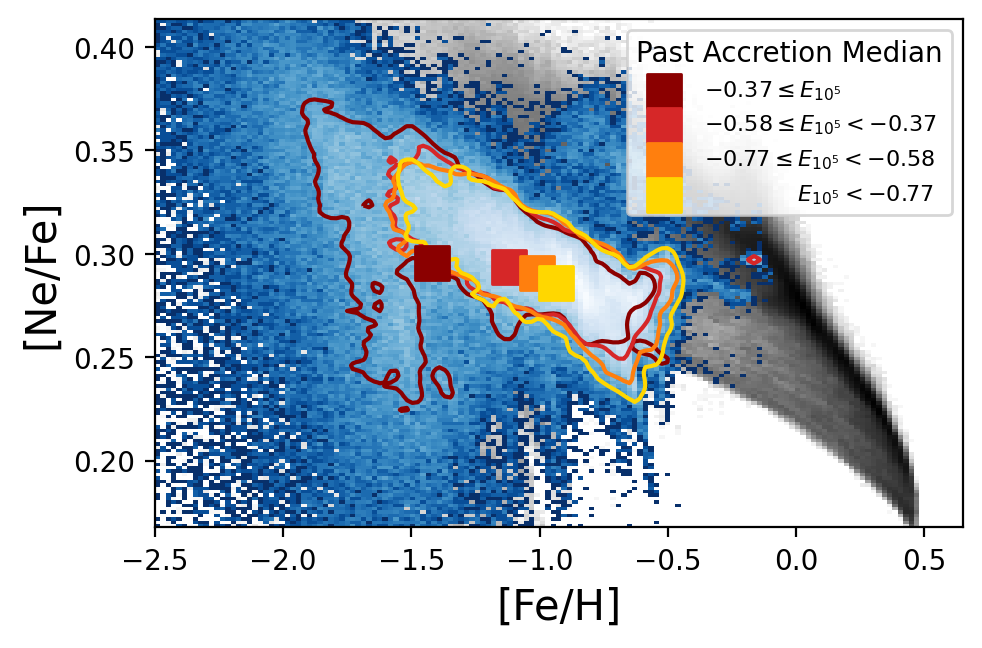
\includegraphics[width=0.33\textwidth]{figures/xfe_feh_zones_Ne.png}
    % Na == Al
    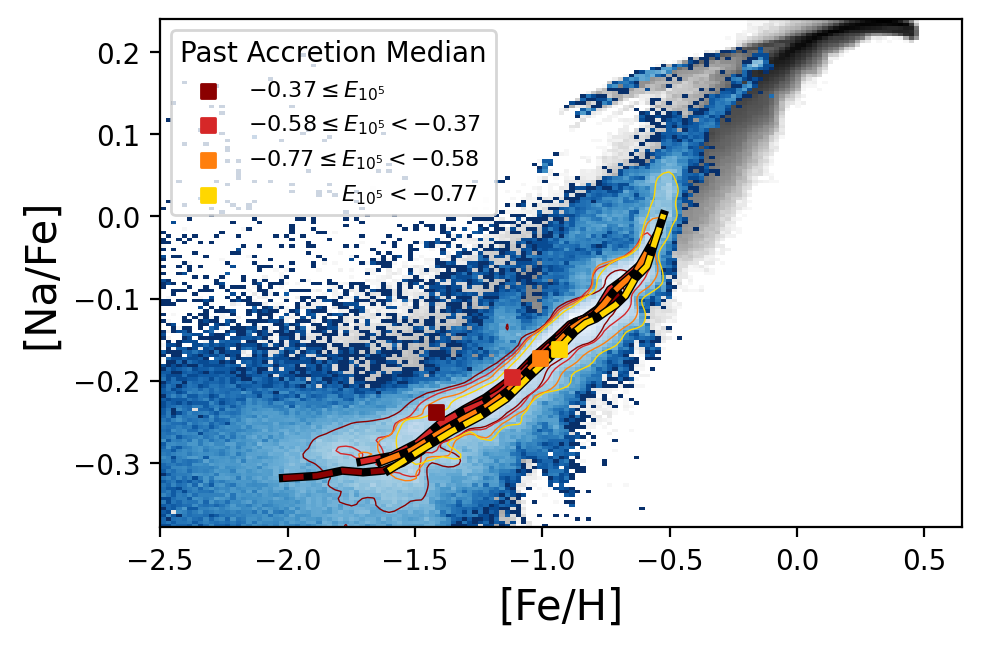
\includegraphics[width=0.33\textwidth]{figures/xfe_feh_zones_Na.png}
    %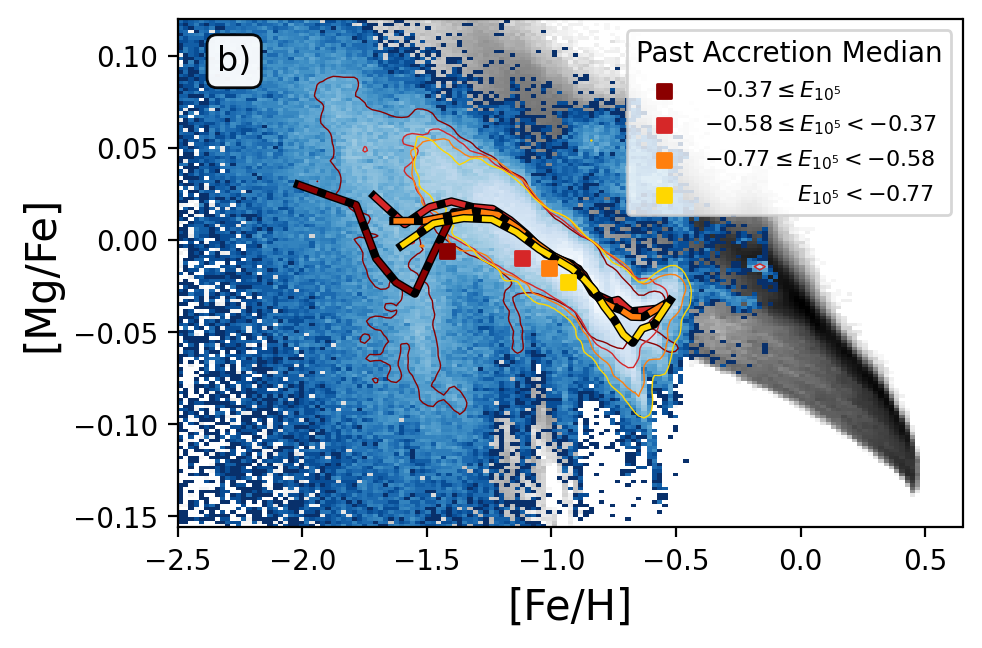
\includegraphics[width=0.33\textwidth]{figures/xfe_feh_zones_Mg.png}
    %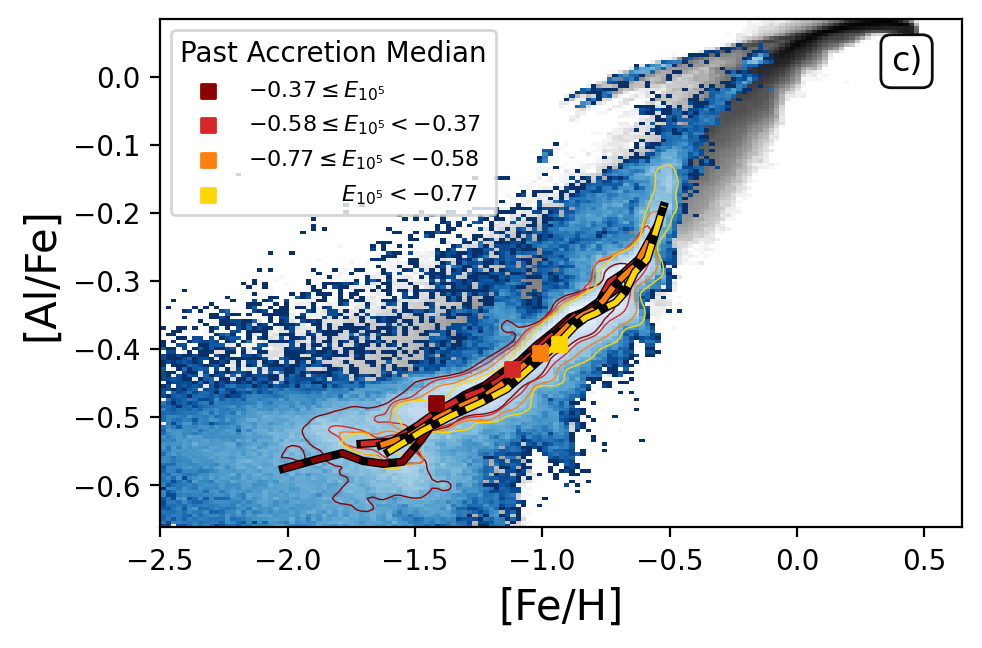
\includegraphics[width=0.33\textwidth]{figures/xfe_feh_zones_Al.png}
    % Si == Mg
    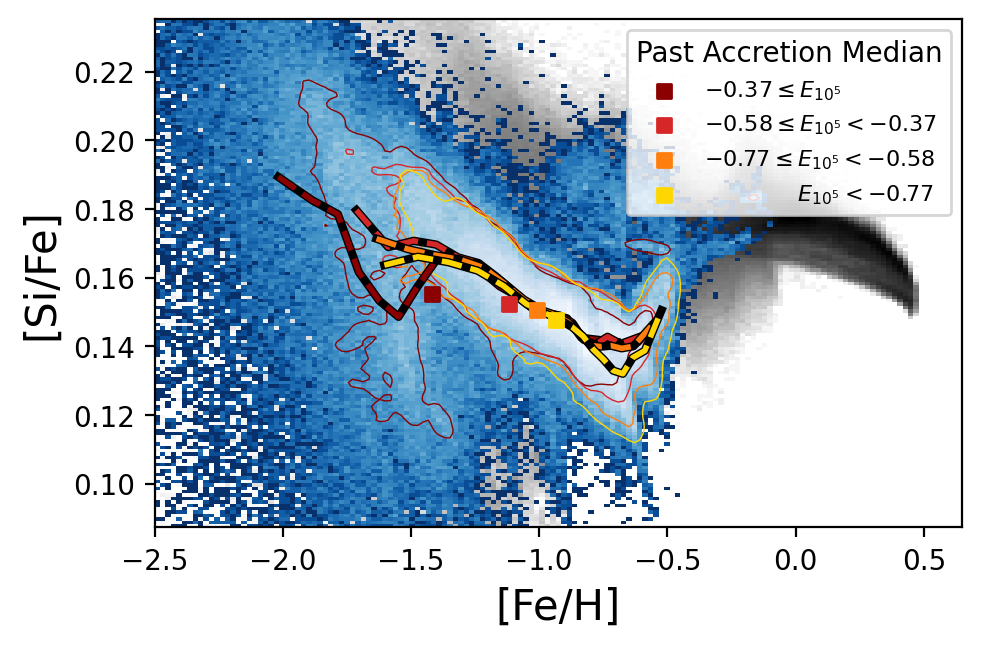
\includegraphics[width=0.33\textwidth]{figures/xfe_feh_zones_Si.png}
    % S == Mg
    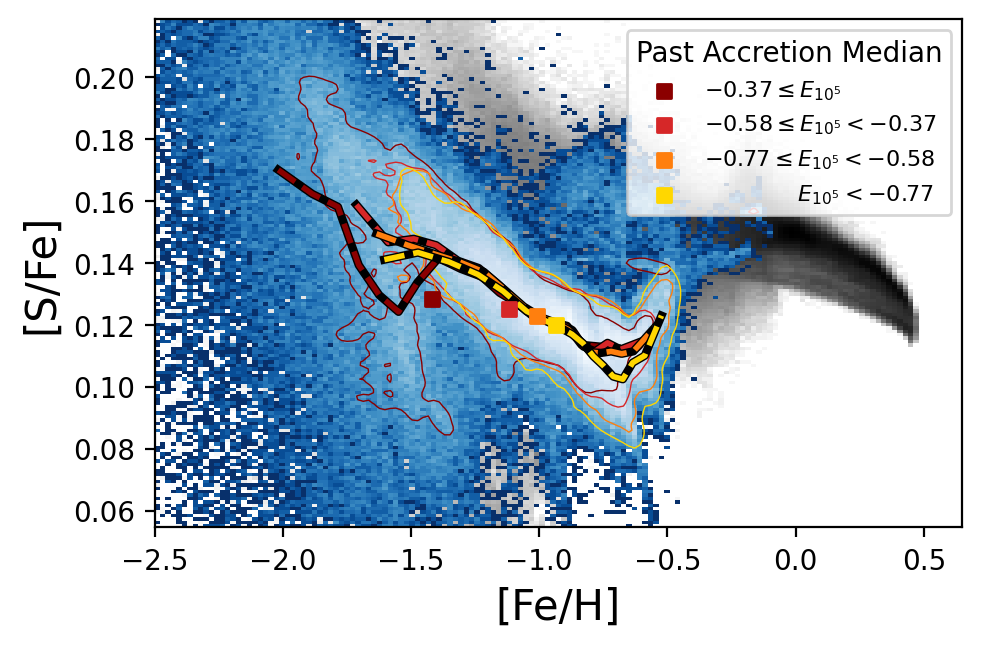
\includegraphics[width=0.33\textwidth]{figures/xfe_feh_zones_S.png}
    % Cl == Al
    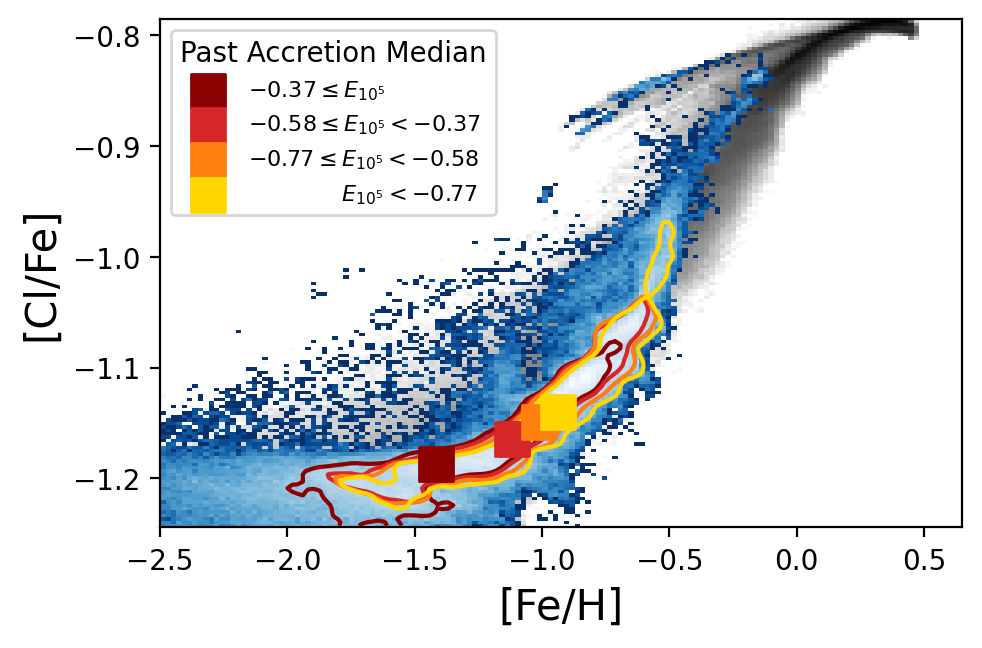
\includegraphics[width=0.33\textwidth]{figures/xfe_feh_zones_Cl.png}
    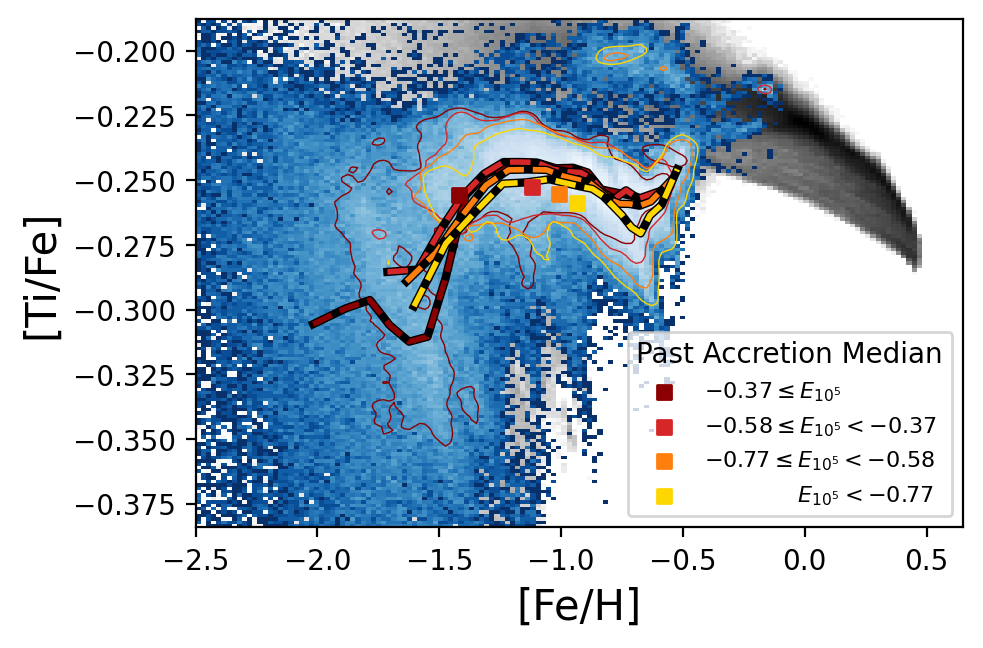
\includegraphics[width=0.33\textwidth]{figures/xfe_feh_zones_Ti.png}
    % Ni == Mn
    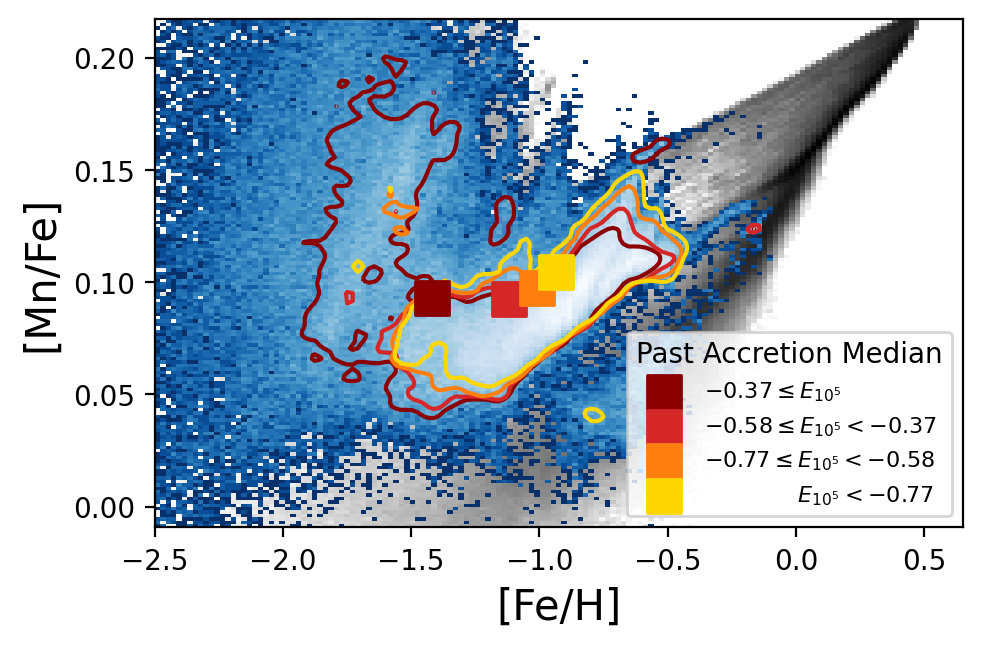
\includegraphics[width=0.33\textwidth]{figures/xfe_feh_zones_Mn.png}
    %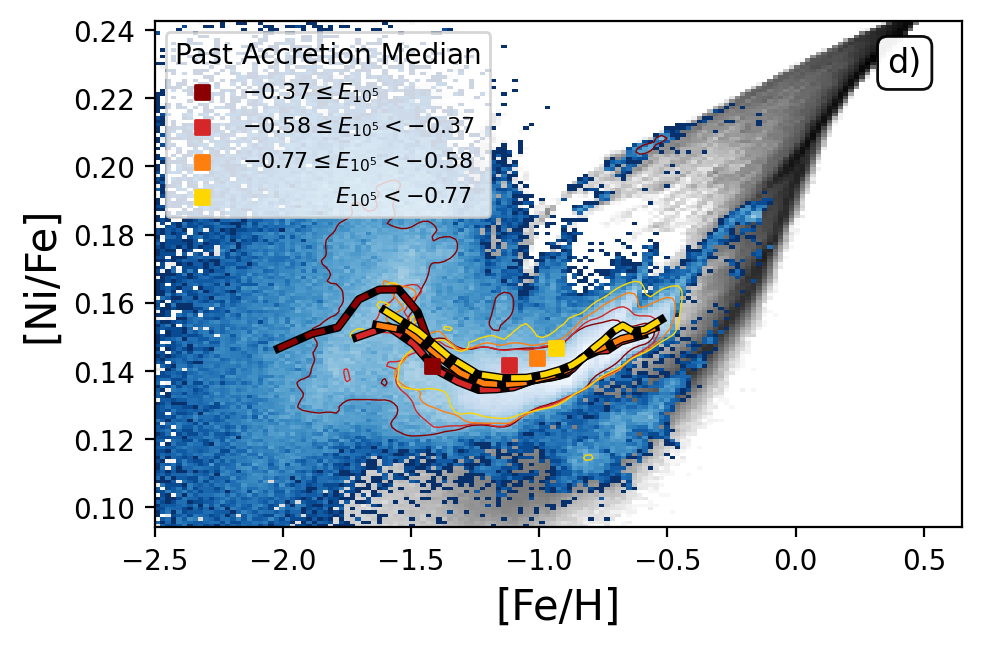
\includegraphics[width=0.33\textwidth]{figures/xfe_feh_zones_Ni.png}
    % Cu == Al
    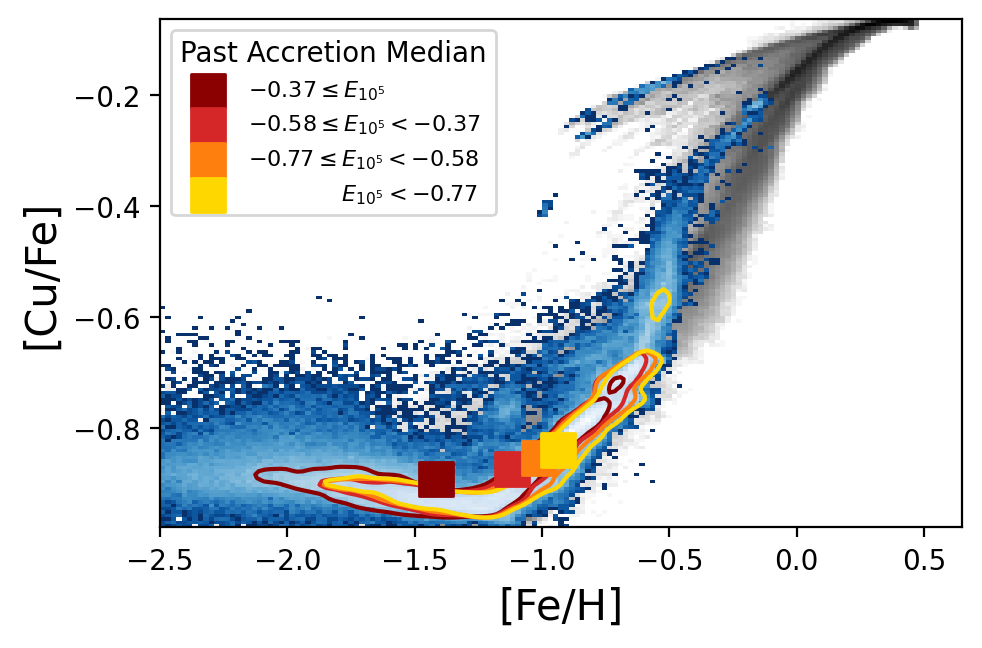
\includegraphics[width=0.33\textwidth]{figures/xfe_feh_zones_Cu.png}
    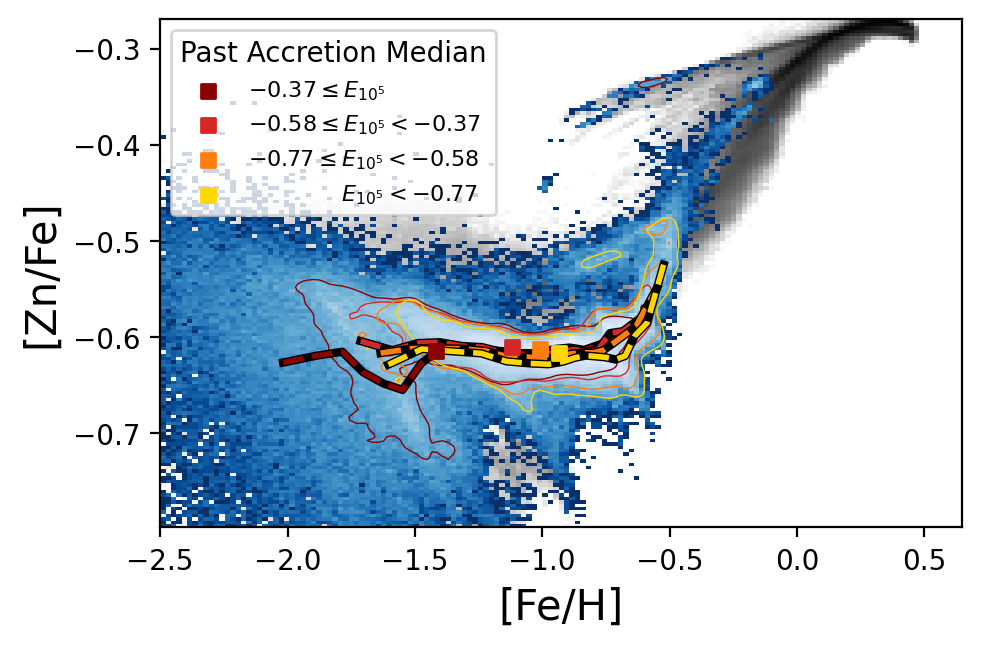
\includegraphics[width=0.33\textwidth]{figures/xfe_feh_zones_Zn.png}
    % Y == Ba
    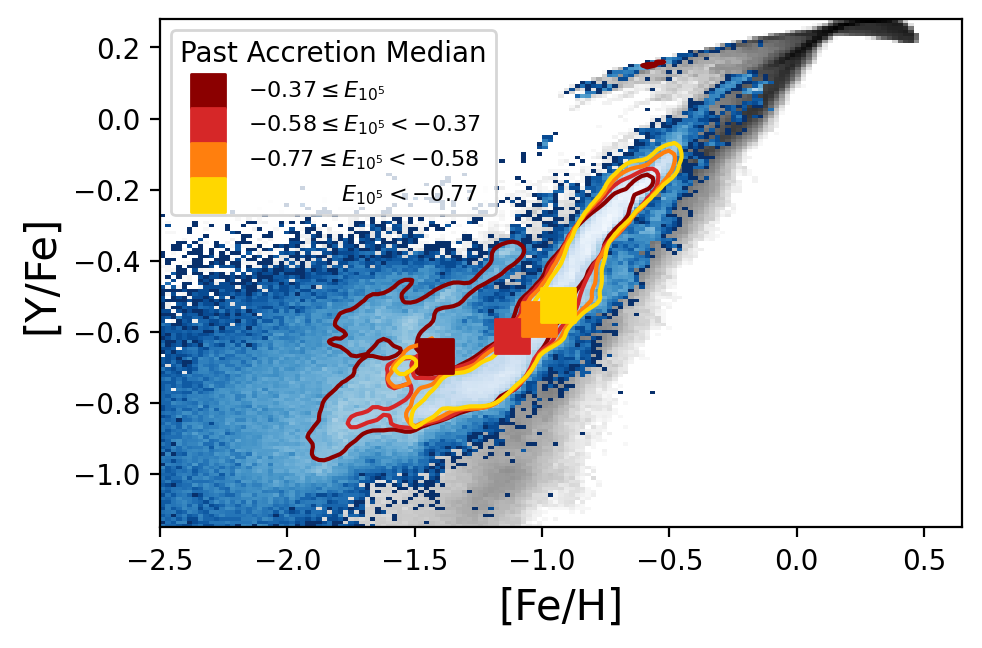
\includegraphics[width=0.33\textwidth]{figures/xfe_feh_zones_Y.png}
    % Ba == Ba
    %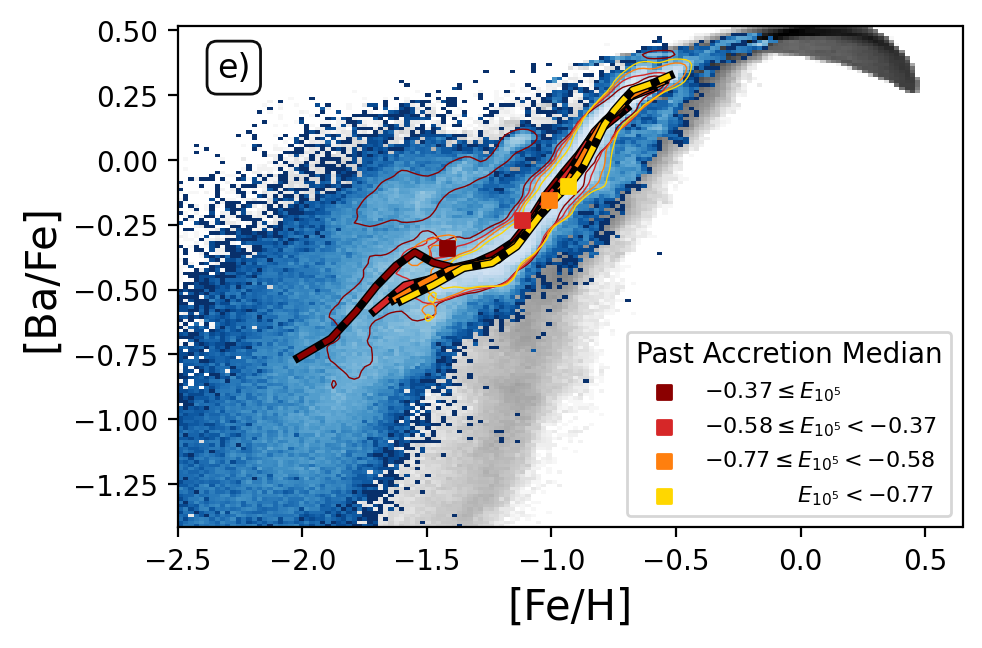
\includegraphics[width=0.33\textwidth]{figures/xfe_feh_zones_Ba.png}
    % Ce == Ba
    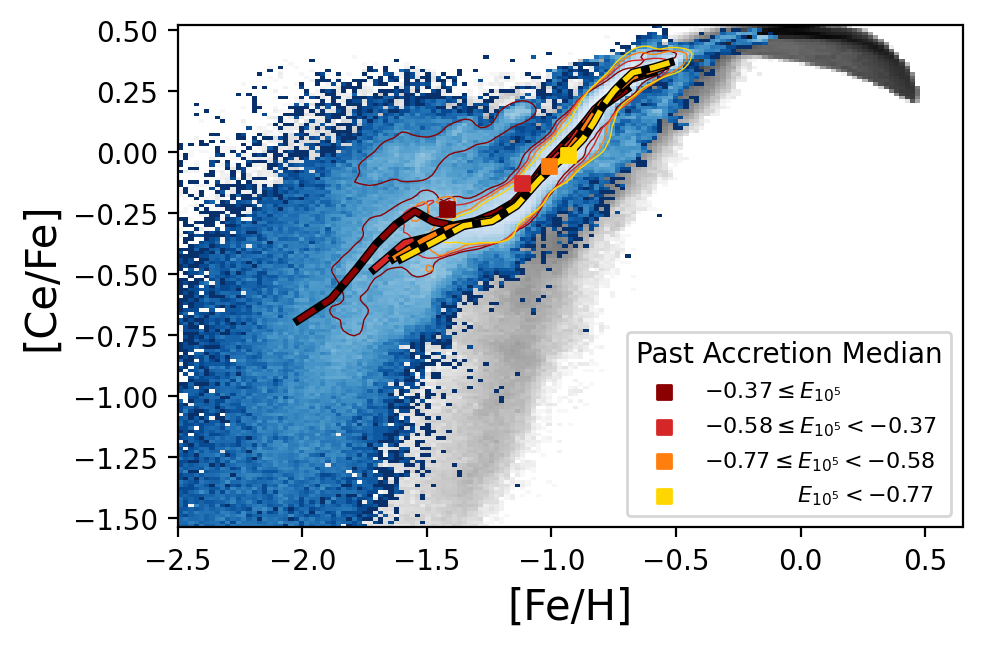
\includegraphics[width=0.33\textwidth]{figures/xfe_feh_zones_Ce.png}
    % Eu == Ba
    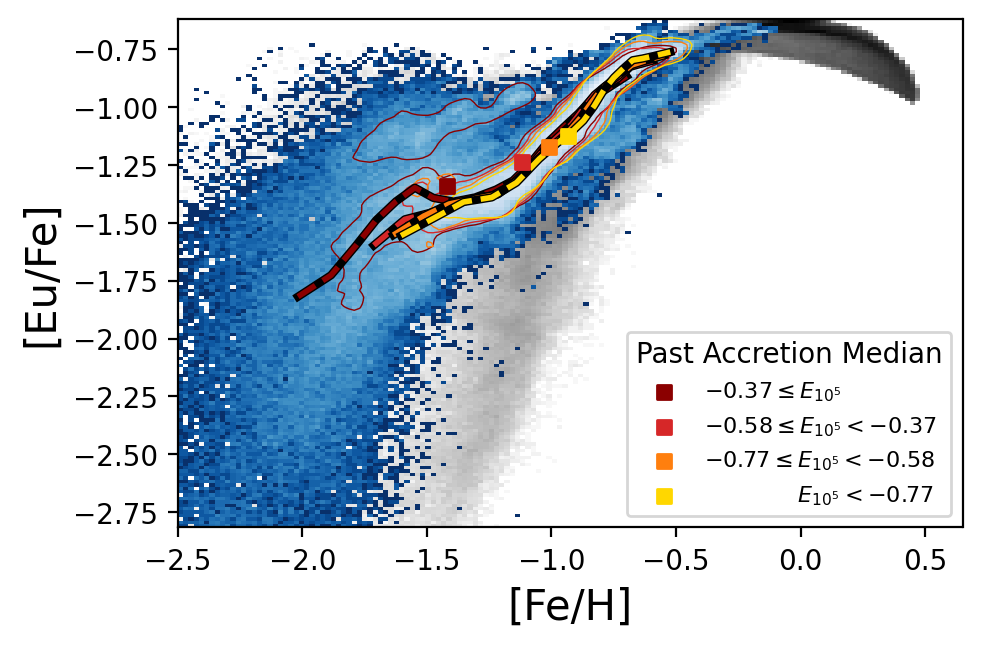
\includegraphics[width=0.33\textwidth]{figures/xfe_feh_zones_Eu.png}
    %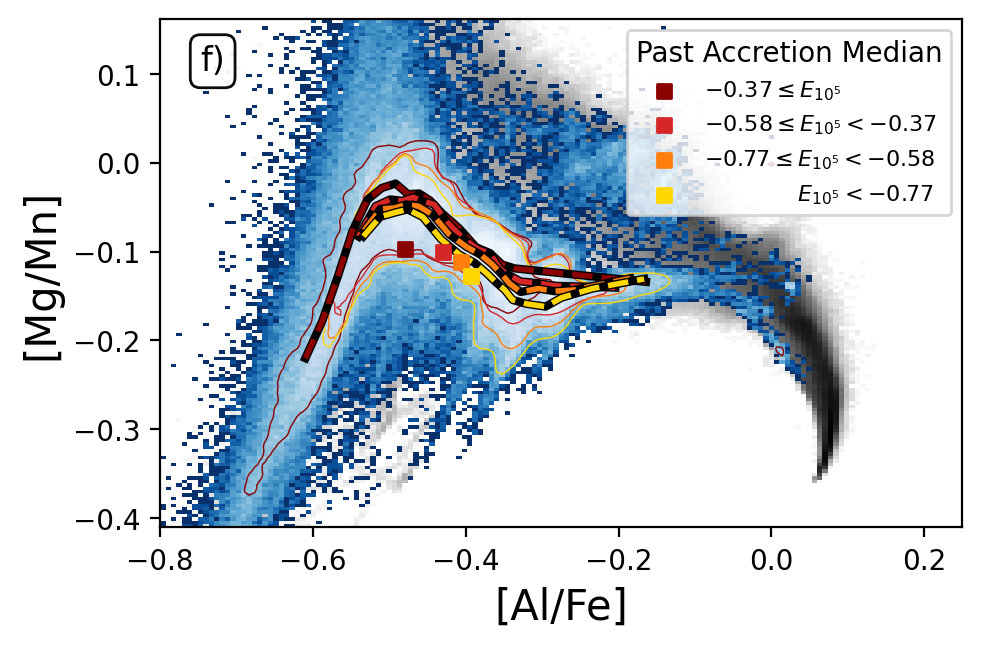
\includegraphics[width=0.33\textwidth]{figures/xfe_feh_zones_MgMn.png}
    \caption{Same as Fig.~\ref{fig:xfe_feh_zones}, for C, N, O, Ne, Na, Si, S, Cl, Ti, Mn, Cu, Zn, Y, Ce, and Eu in the others \href{https://github.com/svenbuder/gse_nihaouhd/tree/main/figures}{\faGithub}.}
    \label{fig:additional_xfe_feh_zones}
\end{figure*}

\bsp
\label{lastpage}
\end{document}